% Options for packages loaded elsewhere
\PassOptionsToPackage{unicode}{hyperref}
\PassOptionsToPackage{hyphens}{url}
%
\documentclass[
  12pt,
]{article}
\usepackage{amsmath,amssymb}
\usepackage{lmodern}
\usepackage{iftex}
\ifPDFTeX
  \usepackage[T1]{fontenc}
  \usepackage[utf8]{inputenc}
  \usepackage{textcomp} % provide euro and other symbols
\else % if luatex or xetex
  \usepackage{unicode-math}
  \defaultfontfeatures{Scale=MatchLowercase}
  \defaultfontfeatures[\rmfamily]{Ligatures=TeX,Scale=1}
\fi
% Use upquote if available, for straight quotes in verbatim environments
\IfFileExists{upquote.sty}{\usepackage{upquote}}{}
\IfFileExists{microtype.sty}{% use microtype if available
  \usepackage[]{microtype}
  \UseMicrotypeSet[protrusion]{basicmath} % disable protrusion for tt fonts
}{}
\usepackage{xcolor}
\usepackage[margin=1in]{geometry}
\usepackage{longtable,booktabs,array}
\usepackage{calc} % for calculating minipage widths
% Correct order of tables after \paragraph or \subparagraph
\usepackage{etoolbox}
\makeatletter
\patchcmd\longtable{\par}{\if@noskipsec\mbox{}\fi\par}{}{}
\makeatother
% Allow footnotes in longtable head/foot
\IfFileExists{footnotehyper.sty}{\usepackage{footnotehyper}}{\usepackage{footnote}}
\makesavenoteenv{longtable}
\usepackage{graphicx}
\makeatletter
\def\maxwidth{\ifdim\Gin@nat@width>\linewidth\linewidth\else\Gin@nat@width\fi}
\def\maxheight{\ifdim\Gin@nat@height>\textheight\textheight\else\Gin@nat@height\fi}
\makeatother
% Scale images if necessary, so that they will not overflow the page
% margins by default, and it is still possible to overwrite the defaults
% using explicit options in \includegraphics[width, height, ...]{}
\setkeys{Gin}{width=\maxwidth,height=\maxheight,keepaspectratio}
% Set default figure placement to htbp
\makeatletter
\def\fps@figure{htbp}
\makeatother
\setlength{\emergencystretch}{3em} % prevent overfull lines
\providecommand{\tightlist}{%
  \setlength{\itemsep}{0pt}\setlength{\parskip}{0pt}}
\setcounter{secnumdepth}{5}
\usepackage{mathptmx} %to use times new roman font
\usepackage[flushleft]{threeparttable}
\usepackage{multirow}
\usepackage{multicol}
\usepackage{booktabs,caption}
\usepackage{pdflscape}
\usepackage{indentfirst}
\usepackage{float}
\usepackage{longtable}
\usepackage{array}
\usepackage{wrapfig}
\usepackage{float}
\usepackage{colortbl}
\usepackage{tabu}
\usepackage{threeparttablex}
\usepackage[normalem]{ulem}
\usepackage{makecell}
\usepackage{xcolor}
\usepackage{siunitx}
\sisetup{round-mode = places, round-precision = 4,}
\interfootnotelinepenalty=10000
\ifLuaTeX
  \usepackage{selnolig}  % disable illegal ligatures
\fi
\IfFileExists{bookmark.sty}{\usepackage{bookmark}}{\usepackage{hyperref}}
\IfFileExists{xurl.sty}{\usepackage{xurl}}{} % add URL line breaks if available
\urlstyle{same} % disable monospaced font for URLs
\hypersetup{
  pdftitle={House Prices and Credit Cycles - Bayesian Regression Results},
  pdfauthor={Nam Nguyen},
  hidelinks,
  pdfcreator={LaTeX via pandoc}}

\title{House Prices and Credit Cycles - Bayesian Regression Results}
\author{Nam Nguyen}
\date{July 18, 2022}

\begin{document}
\maketitle

\hypertarget{description}{%
\section{Description}\label{description}}

The following Baysian regression implementation is based on Metropolis-Hasting random walk algorithm from Chapter 5 - Applied Bayesian econometrics for Central Bankers. The posterior results are summarized from 1,500,000 iterations with the first 500,000 iterations discarded for each model.

\hypertarget{regression-results}{%
\section{REGRESSION RESULTS}\label{regression-results}}

        \begin{table}[H]
            \begin{threeparttable}
                \caption {\label{tab:table1} Parameters description}
                %\rowcolors{2}{gray!10}{white} 
                \begin{tabular}{@{}ll@{}}
                    \toprule
                    Description & Parameter\\
                    \midrule
                    Log-likelihood value & $llv$ \\[2pt] 
                    Credit to household & \\
                    \quad Credit to household 1st AR parameter  & $\phi^1_{y}$ \\[2pt] 
                    \quad Credit to household 2nd AR parameter  & $\phi^2_{y}$ \\[2pt] 
                    \quad Credit to household 1st cross cycle AR parameter  & $\phi^{x1}_{y}$ \\[2pt] 
                    \quad Credit to household 2nd cross cycle AR parameter  & $\phi^{x2}_{y}$ \\[2pt] 
                    \quad S.D. of permanent shocks to Credit to household & $\sigma_{ny}$ \\[2pt] 
                    \quad S.D. of transitory shocks to Credit to household & $\sigma_{ey}$ \\[2pt]
                    Housing Price Index & \\
                    \quad Housing Price Index 1st AR parameter  & $\phi^1_{h}$ \\[2pt] 
                    \quad Housing Price Index 2nd AR parameter  & $\phi^2_{h}$ \\[2pt] 
                    \quad Housing Price Index 1st cross cycle AR parameter  & $\phi^{x1}_{h}$ \\[2pt] 
                    \quad Housing Price Index 2nd cross cycle AR parameter  & $\phi^{x2}_{h}$ \\[2pt] 
                    \quad S.D. of permanent shocks to Housing Price Index & $\sigma_{nh}$ \\[2pt] 
                    \quad S.D. of transitory shocks to Housing Price Index & $\sigma_{eh}$ \\[2pt]
                    Cross-series correlations & \\
                    \quad Correlation: Permanent credit to household/Permanent Housing Price Index  & $\rho_{nynh}$ \\[2pt] 
                    \quad Correlation: Transitory credit to household/Transitory Housing Price Index  & $\rho_{eyeh}$ \\[2pt] 
                                        
                    \bottomrule
                \end{tabular}
%               \begin{tablenotes}
%                   \small
%                   \item $y_t$ is credit to household series, $h_t$ is housing price index series. Both are log transformed. \\
%               \end{tablenotes}
            \end{threeparttable}
        \end{table}

\begin{landscape}

\begin{table}

\caption{\label{tab:unnamed-chunk-1}UK Regression Results}
\centering
\resizebox{\linewidth}{!}{
\begin{tabular}[t]{>{}l>{}lrl>{}r>{}lrl}
\toprule
\multicolumn{2}{c}{ } & \multicolumn{2}{c}{VAR2} & \multicolumn{2}{c}{VAR2 1-cross lag} & \multicolumn{2}{c}{VAR2 2-cross lags} \\
\cmidrule(l{3pt}r{3pt}){3-4} \cmidrule(l{3pt}r{3pt}){5-6} \cmidrule(l{3pt}r{3pt}){7-8}
Description & Parameters & Median & {}[10$\%$, 90$\%$] & Median & {}[10$\%$, 90$\%$] & Median & {}[10$\%$, 90$\%$]\\
\midrule
\cellcolor{gray!6}{Credit to household 1st AR parameter} & \cellcolor{gray!6}{$\phi^1_{y}$} & \cellcolor{gray!6}{1.9827} & \cellcolor{gray!6}{{}[1.9770, 1.9898]} & \cellcolor{gray!6}{1.4238} & \cellcolor{gray!6}{{}[1.3585, 1.4892]} & \cellcolor{gray!6}{1.4354} & \cellcolor{gray!6}{{}[1.3627, 1.5080]}\\
Credit to household 2nd AR parameter & $\phi^2_{y}$ & -1.0056 & {}[-1.0126, -0.9985] & -0.4698 & {}[-0.5305, -0.4090] & -0.4946 & {}[-0.5599, -0.4301]\\
\textbf{\cellcolor{gray!6}{Credit to household 1st cross cycle AR parameter}} & \textbf{\cellcolor{gray!6}{$\phi^{x1}_{y}$}} & \cellcolor{gray!6}{} & \cellcolor{gray!6}{} & \textbf{\cellcolor{gray!6}{0.0238}} & \textbf{\cellcolor{gray!6}{{}[0.0154, 0.0319]}} & \cellcolor{gray!6}{0.0023} & \cellcolor{gray!6}{{}[-0.0208, 0.0257]}\\
Credit to household 2nd cross cycle AR parameter & $\phi^{x2}_{y}$ &  &  &  &  & 0.0165 & {}[-0.0075, 0.0399]\\
\addlinespace
\cellcolor{gray!6}{Housing Price Index 1st AR parameter} & \cellcolor{gray!6}{$\phi^1_{h}$} & \cellcolor{gray!6}{1.4119} & \cellcolor{gray!6}{{}[1.3987, 1.4238]} & \cellcolor{gray!6}{1.3173} & \cellcolor{gray!6}{{}[1.2647, 1.3701]} & \cellcolor{gray!6}{1.2844} & \cellcolor{gray!6}{{}[1.2233, 1.3458]}\\
Housing Price Index 2nd AR parameter & $\phi^2_{h}$ & -0.4323 & {}[-0.4464, -0.4227] & -0.3315 & {}[-0.3885, -0.2746] & -0.3041 & {}[-0.3686, -0.2409]\\
\textbf{\cellcolor{gray!6}{Housing Price Index 1st cross cycle AR parameter}} & \textbf{\cellcolor{gray!6}{$\phi^{x1}_{h}$}} & \cellcolor{gray!6}{} & \cellcolor{gray!6}{} & \textbf{\cellcolor{gray!6}{-0.0173}} & \textbf{\cellcolor{gray!6}{{}[-0.0464, 0.0062]}} & \cellcolor{gray!6}{0.4847} & \cellcolor{gray!6}{{}[0.2707, 0.6894]}\\
Housing Price Index 2nd cross cycle AR parameter & $\phi^{x2}_{h}$ &  &  &  &  & -0.4960 & {}[-0.6698, -0.3198]\\
\addlinespace
\cellcolor{gray!6}{S.D. of permanent shocks to Credit to household} & \cellcolor{gray!6}{$\sigma_{ny}$} & \cellcolor{gray!6}{0.1055} & \cellcolor{gray!6}{{}[0.0896, 0.1254]} & \cellcolor{gray!6}{0.2714} & \cellcolor{gray!6}{{}[0.2150, 0.3155]} & \cellcolor{gray!6}{0.0737} & \cellcolor{gray!6}{{}[0.0463, 0.0987]}\\
S.D. of transitory shocks to Credit to household & $\sigma_{ey}$ & 0.8113 & {}[0.7957, 0.8259] & 0.8021 & {}[0.7699, 0.8376] & 0.6336 & {}[0.5803, 0.6925]\\
\cellcolor{gray!6}{S.D. of permanent shocks to Housing Price Index} & \cellcolor{gray!6}{$\sigma_{nh}$} & \cellcolor{gray!6}{0.0062} & \cellcolor{gray!6}{{}[0.0055, 0.0072]} & \cellcolor{gray!6}{0.0789} & \cellcolor{gray!6}{{}[0.0742, 0.0845]} & \cellcolor{gray!6}{0.0062} & \cellcolor{gray!6}{{}[0.0055, 0.0071]}\\
S.D. of transitory shocks to Housing Price Index & $\sigma_{eh}$ & 1.8647 & {}[1.8332, 1.8845] & 1.2242 & {}[1.1886, 1.2613] & 1.5020 & {}[1.4080, 1.6063]\\
\addlinespace
\cellcolor{gray!6}{Correlation: Permanent credit to household$\slash$Permanent HPI} & \cellcolor{gray!6}{$\rho_{nynh}$} & \cellcolor{gray!6}{0.0589} & \cellcolor{gray!6}{{}[0.0418, 0.0808]} & \cellcolor{gray!6}{0.0189} & \cellcolor{gray!6}{{}[-0.3049, 0.3393]} & \cellcolor{gray!6}{0.0150} & \cellcolor{gray!6}{{}[-0.3101, 0.3306]}\\
Correlation: Transitory credit to household$\slash$Transitory HPI & $\rho_{eyeh}$ & 0.3373 & {}[0.2938, 0.3485] & 0.2536 & {}[0.1713, 0.3337] & 0.2533 & {}[0.1582, 0.3426]\\
\cellcolor{gray!6}{Log-likelihood value} & \cellcolor{gray!6}{$llv$} & \cellcolor{gray!6}{607.7600} & \cellcolor{gray!6}{{}[605.0700, 610.0600]} & \cellcolor{gray!6}{578.6200} & \cellcolor{gray!6}{{}[576.1600, 582.1500]} & \cellcolor{gray!6}{559.5500} & \cellcolor{gray!6}{{}[556.6400, 563.6200]}\\
\bottomrule
\multicolumn{8}{l}{\rule{0pt}{1em}\textit{Note: }}\\
\multicolumn{8}{l}{\rule{0pt}{1em}UK Bayesian regression results}\\
\end{tabular}}
\end{table}
\end{landscape}

\clearpage

\begin{landscape}

\begin{table}

\caption{\label{tab:unnamed-chunk-2}US Regression Results}
\centering
\resizebox{\linewidth}{!}{
\begin{tabular}[t]{>{}l>{}lrl>{}r>{}lrl}
\toprule
\multicolumn{2}{c}{ } & \multicolumn{2}{c}{VAR2} & \multicolumn{2}{c}{VAR2 1-cross lag} & \multicolumn{2}{c}{VAR2 2-cross lags} \\
\cmidrule(l{3pt}r{3pt}){3-4} \cmidrule(l{3pt}r{3pt}){5-6} \cmidrule(l{3pt}r{3pt}){7-8}
Description & Parameters & Median & {}[10$\%$, 90$\%$] & Median & {}[10$\%$, 90$\%$] & Median & {}[10$\%$, 90$\%$]\\
\midrule
\cellcolor{gray!6}{Credit to household 1st AR parameter} & \cellcolor{gray!6}{$\phi^1_{y}$} & \cellcolor{gray!6}{1.4826} & \cellcolor{gray!6}{{}[1.4216, 1.5446]} & \cellcolor{gray!6}{1.2074} & \cellcolor{gray!6}{{}[1.1374, 1.2785]} & \cellcolor{gray!6}{1.2004} & \cellcolor{gray!6}{{}[1.1227, 1.2753]}\\
Credit to household 2nd AR parameter & $\phi^2_{y}$ & -0.4887 & {}[-0.5500, -0.4280] & -0.2483 & {}[-0.3152, -0.1825] & -0.2554 & {}[-0.3209, -0.1884]\\
\textbf{\cellcolor{gray!6}{Credit to household 1st cross cycle AR parameter}} & \textbf{\cellcolor{gray!6}{$\phi^{x1}_{y}$}} & \cellcolor{gray!6}{} & \cellcolor{gray!6}{} & \textbf{\cellcolor{gray!6}{0.0318}} & \textbf{\cellcolor{gray!6}{{}[0.0228, 0.0407]}} & \cellcolor{gray!6}{0.0380} & \cellcolor{gray!6}{{}[0.0003, 0.0732]}\\
Credit to household 2nd cross cycle AR parameter & $\phi^{x2}_{y}$ &  &  &  &  & -0.0088 & {}[-0.0451, 0.0297]\\
\addlinespace
\cellcolor{gray!6}{Housing Price Index 1st AR parameter} & \cellcolor{gray!6}{$\phi^1_{h}$} & \cellcolor{gray!6}{1.8594} & \cellcolor{gray!6}{{}[1.8276, 1.8915]} & \cellcolor{gray!6}{1.8038} & \cellcolor{gray!6}{{}[1.7700, 1.8363]} & \cellcolor{gray!6}{1.7999} & \cellcolor{gray!6}{{}[1.7658, 1.8345]}\\
Housing Price Index 2nd AR parameter & $\phi^2_{h}$ & -0.8728 & {}[-0.9047, -0.8408] & -0.8261 & {}[-0.8605, -0.7903] & -0.8316 & {}[-0.8687, -0.7942]\\
\textbf{\cellcolor{gray!6}{Housing Price Index 1st cross cycle AR parameter}} & \textbf{\cellcolor{gray!6}{$\phi^{x1}_{h}$}} & \cellcolor{gray!6}{} & \cellcolor{gray!6}{} & \textbf{\cellcolor{gray!6}{0.0104}} & \textbf{\cellcolor{gray!6}{{}[0.0007, 0.0204]}} & \cellcolor{gray!6}{0.3305} & \cellcolor{gray!6}{{}[0.2535, 0.4066]}\\
Housing Price Index 2nd cross cycle AR parameter & $\phi^{x2}_{h}$ &  &  &  &  & -0.2882 & {}[-0.3584, -0.2163]\\
\addlinespace
\cellcolor{gray!6}{S.D. of permanent shocks to Credit to household} & \cellcolor{gray!6}{$\sigma_{ny}$} & \cellcolor{gray!6}{0.0942} & \cellcolor{gray!6}{{}[0.0558, 0.1285]} & \cellcolor{gray!6}{0.2954} & \cellcolor{gray!6}{{}[0.2312, 0.3414]} & \cellcolor{gray!6}{0.0853} & \cellcolor{gray!6}{{}[0.0530, 0.1136]}\\
S.D. of transitory shocks to Credit to household & $\sigma_{ey}$ & 0.8282 & {}[0.7616, 0.9059] & 0.8631 & {}[0.8287, 0.9012] & 0.7278 & {}[0.6672, 0.7955]\\
\cellcolor{gray!6}{S.D. of permanent shocks to Housing Price Index} & \cellcolor{gray!6}{$\sigma_{nh}$} & \cellcolor{gray!6}{0.0193} & \cellcolor{gray!6}{{}[0.0150, 0.0265]} & \cellcolor{gray!6}{0.1390} & \cellcolor{gray!6}{{}[0.1222, 0.1618]} & \cellcolor{gray!6}{0.0190} & \cellcolor{gray!6}{{}[0.0147, 0.0258]}\\
S.D. of transitory shocks to Housing Price Index & $\sigma_{eh}$ & 0.8360 & {}[0.7713, 0.9111] & 0.8988 & {}[0.8641, 0.9355] & 0.8001 & {}[0.7321, 0.8735]\\
\addlinespace
\cellcolor{gray!6}{Correlation: Permanent credit to household$\slash$Permanent HPI} & \cellcolor{gray!6}{$\rho_{nynh}$} & \cellcolor{gray!6}{0.0082} & \cellcolor{gray!6}{{}[-0.3118, 0.3230]} & \cellcolor{gray!6}{0.0082} & \cellcolor{gray!6}{{}[-0.3117, 0.3226]} & \cellcolor{gray!6}{0.0167} & \cellcolor{gray!6}{{}[-0.2998, 0.3328]}\\
Correlation: Transitory credit to household$\slash$Transitory HPI & $\rho_{eyeh}$ & 0.1000 & {}[-0.0181, 0.2185] & 0.1537 & {}[0.0399, 0.2619] & 0.1642 & {}[0.0460, 0.2764]\\
\cellcolor{gray!6}{Log-likelihood value} & \cellcolor{gray!6}{$llv$} & \cellcolor{gray!6}{197.7900} & \cellcolor{gray!6}{{}[195.5700, 201.0700]} & \cellcolor{gray!6}{204.9400} & \cellcolor{gray!6}{{}[202.4200, 208.4500]} & \cellcolor{gray!6}{187.7900} & \cellcolor{gray!6}{{}[184.8500, 192.1700]}\\
\bottomrule
\multicolumn{8}{l}{\rule{0pt}{1em}\textit{Note: }}\\
\multicolumn{8}{l}{\rule{0pt}{1em}UK Bayesian regression results}\\
\end{tabular}}
\end{table}
\end{landscape}

\clearpage

\hypertarget{trend-cycle-decompositon-graphs}{%
\section{Trend-Cycle Decompositon Graphs}\label{trend-cycle-decompositon-graphs}}

\hypertarget{uk-graphs}{%
\subsection{UK graphs}\label{uk-graphs}}

\begin{figure}

{\centering 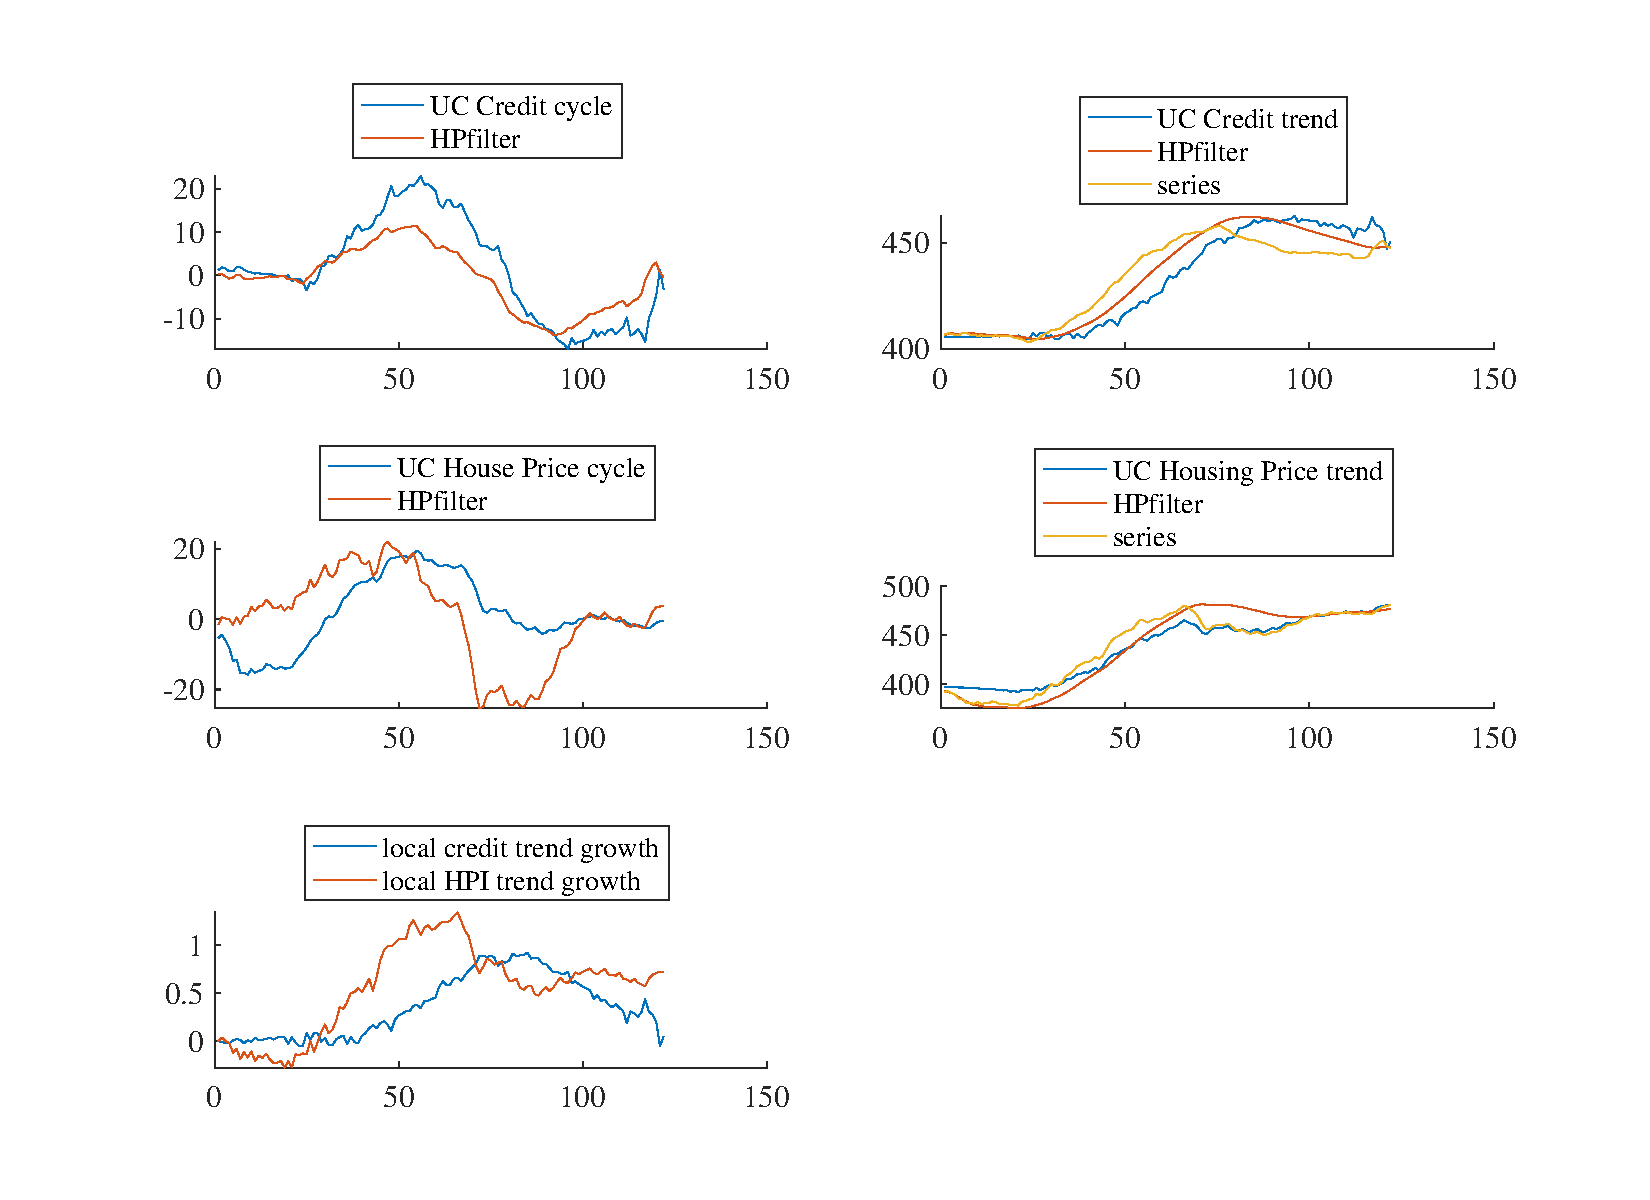
\includegraphics[width=0.85\linewidth]{../../Regression/Bayesian_UC_VAR2_drift/OutputData/cycles_UK} 

}

\caption{UK VAR(2)}\label{fig:unnamed-chunk-3}
\end{figure}

\begin{figure}

{\centering 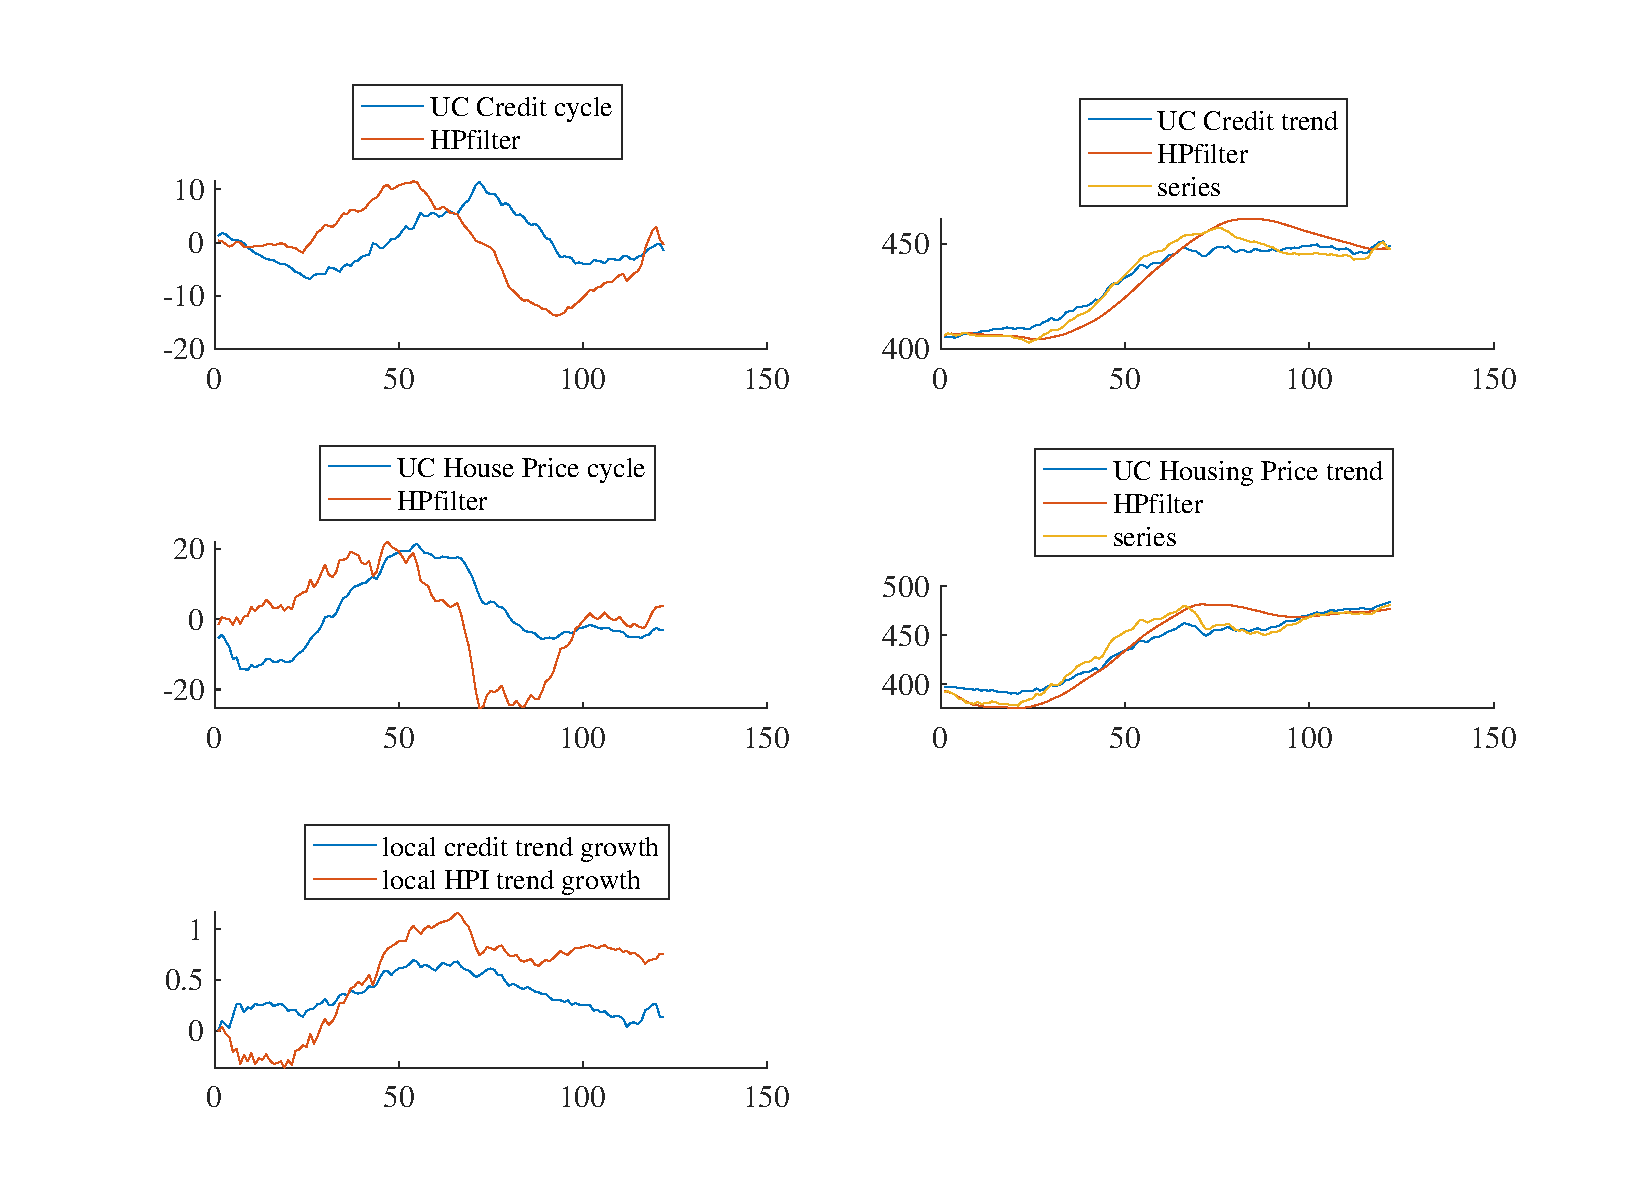
\includegraphics[width=0.85\linewidth]{../../Regression/Bayesian_UC_VAR2_drift_Crosscycle1lag/OutputData/cycles_UK} 

}

\caption{UK VAR(2) 1 cross-lag}\label{fig:unnamed-chunk-4}
\end{figure}

\begin{figure}

{\centering 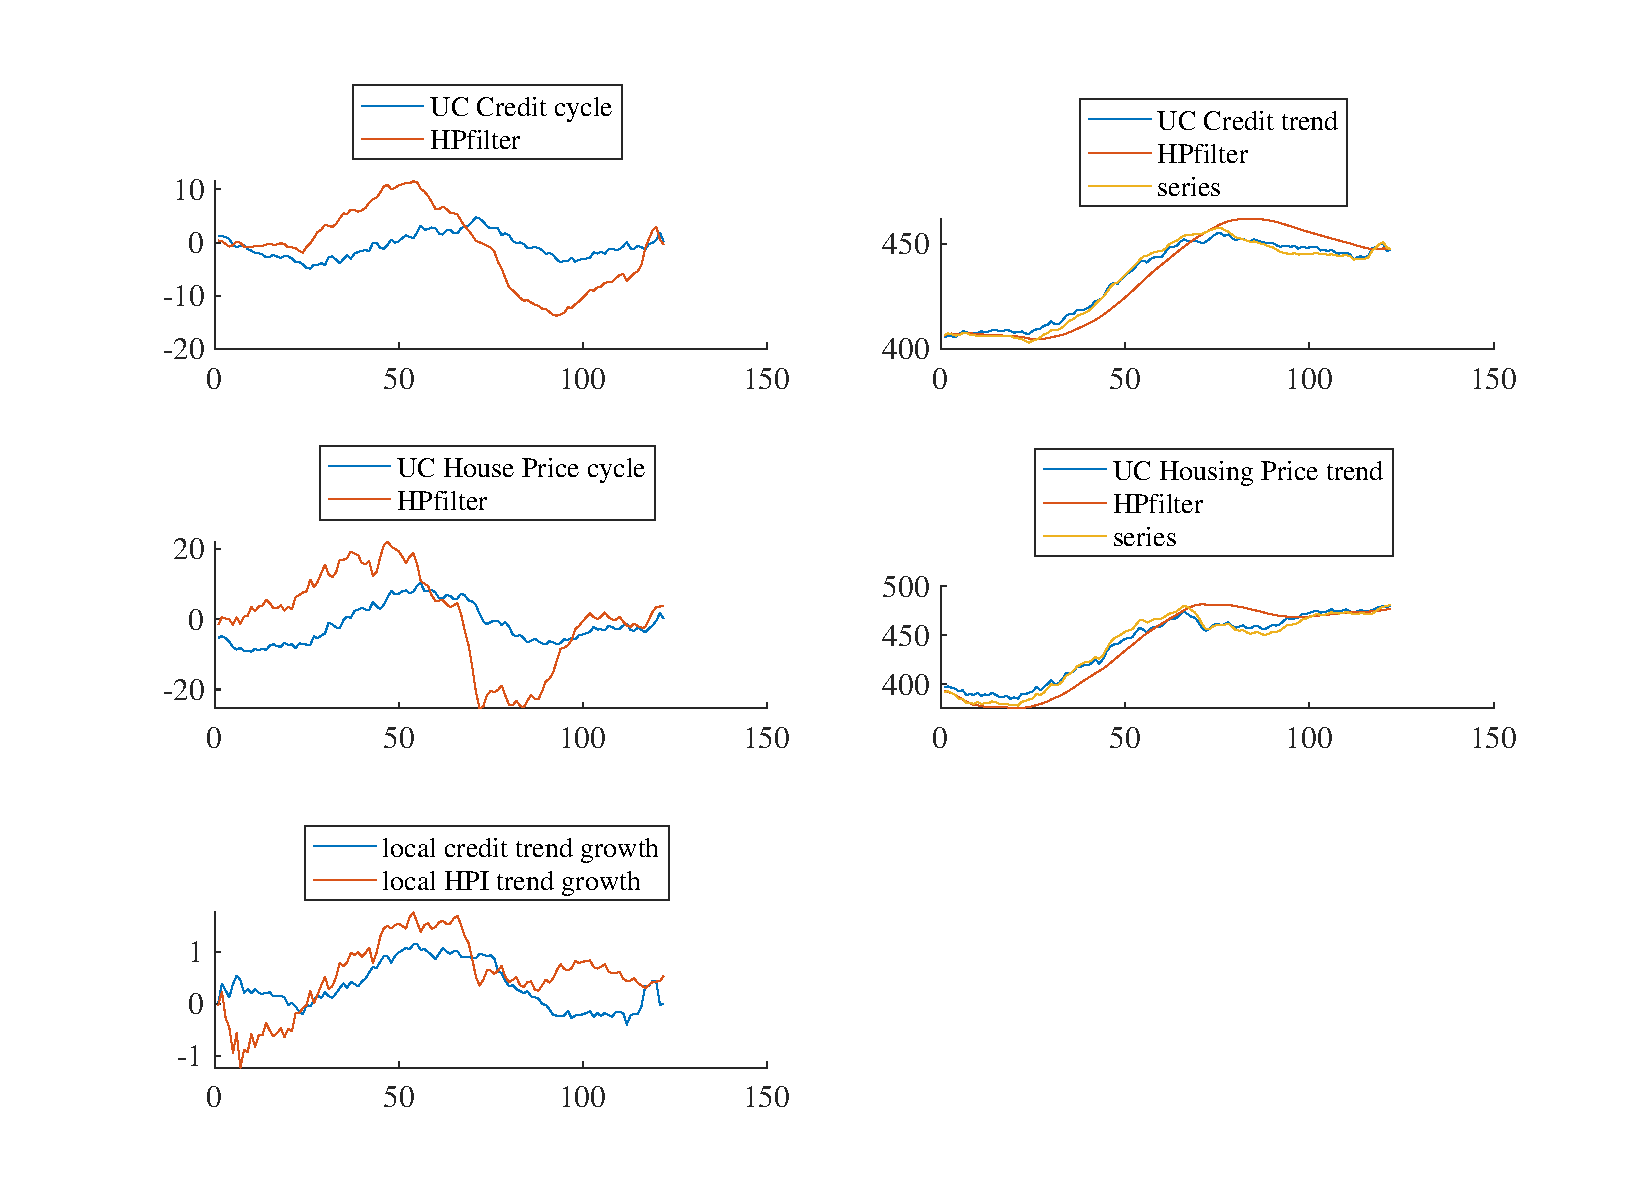
\includegraphics[width=0.85\linewidth]{../../Regression/Bayesian_UC_VAR2_drift_Crosscycle2lags/OutputData/cycles_UK} 

}

\caption{UK VAR(2) 2 cross-lags}\label{fig:unnamed-chunk-5}
\end{figure}

\clearpage

\hypertarget{us-graphs}{%
\subsection{US graphs}\label{us-graphs}}

\begin{figure}

{\centering 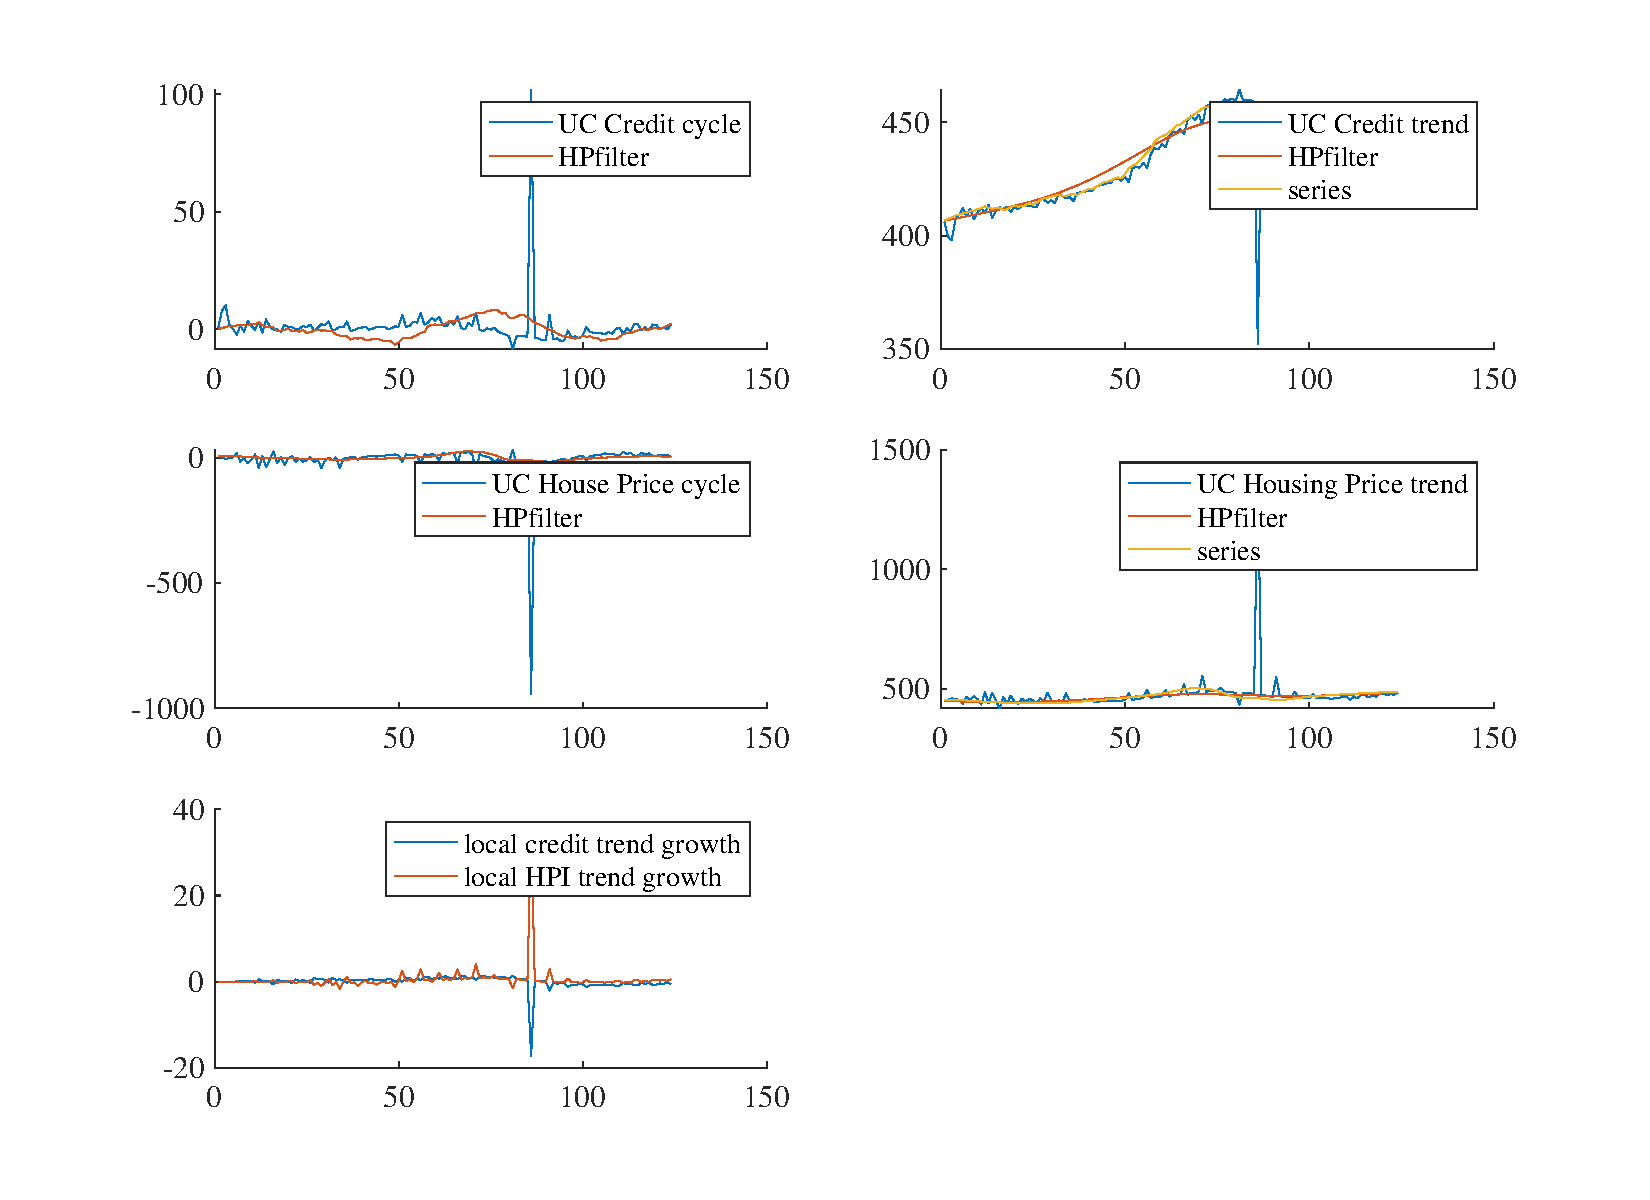
\includegraphics[width=0.85\linewidth]{../../Regression/Bayesian_UC_VAR2_drift/OutputData/cycles_US} 

}

\caption{US VAR(2)}\label{fig:unnamed-chunk-6}
\end{figure}

\begin{figure}

{\centering 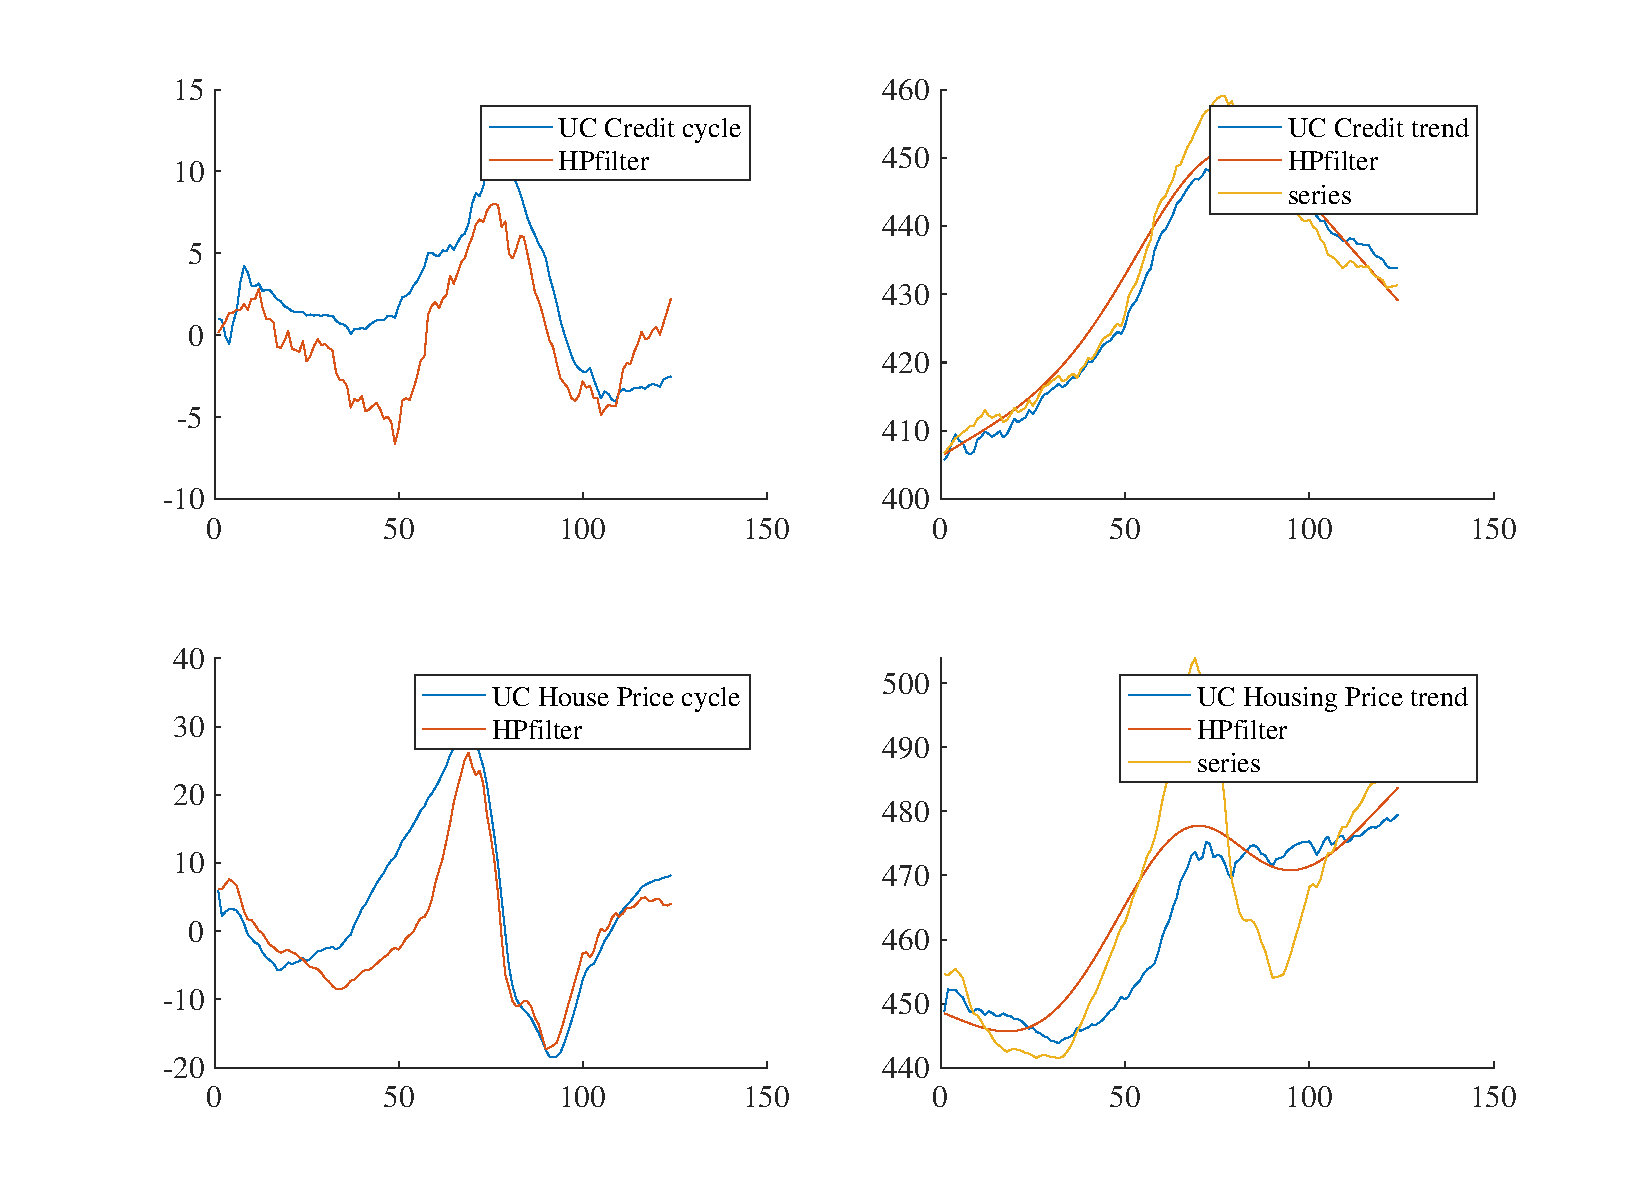
\includegraphics[width=0.85\linewidth]{../../Regression/Bayesian_UC_VAR2_drift_Crosscycle1lag/OutputData/cycles_US} 

}

\caption{US VAR(2) 1 cross-lag}\label{fig:unnamed-chunk-7}
\end{figure}

\begin{figure}

{\centering 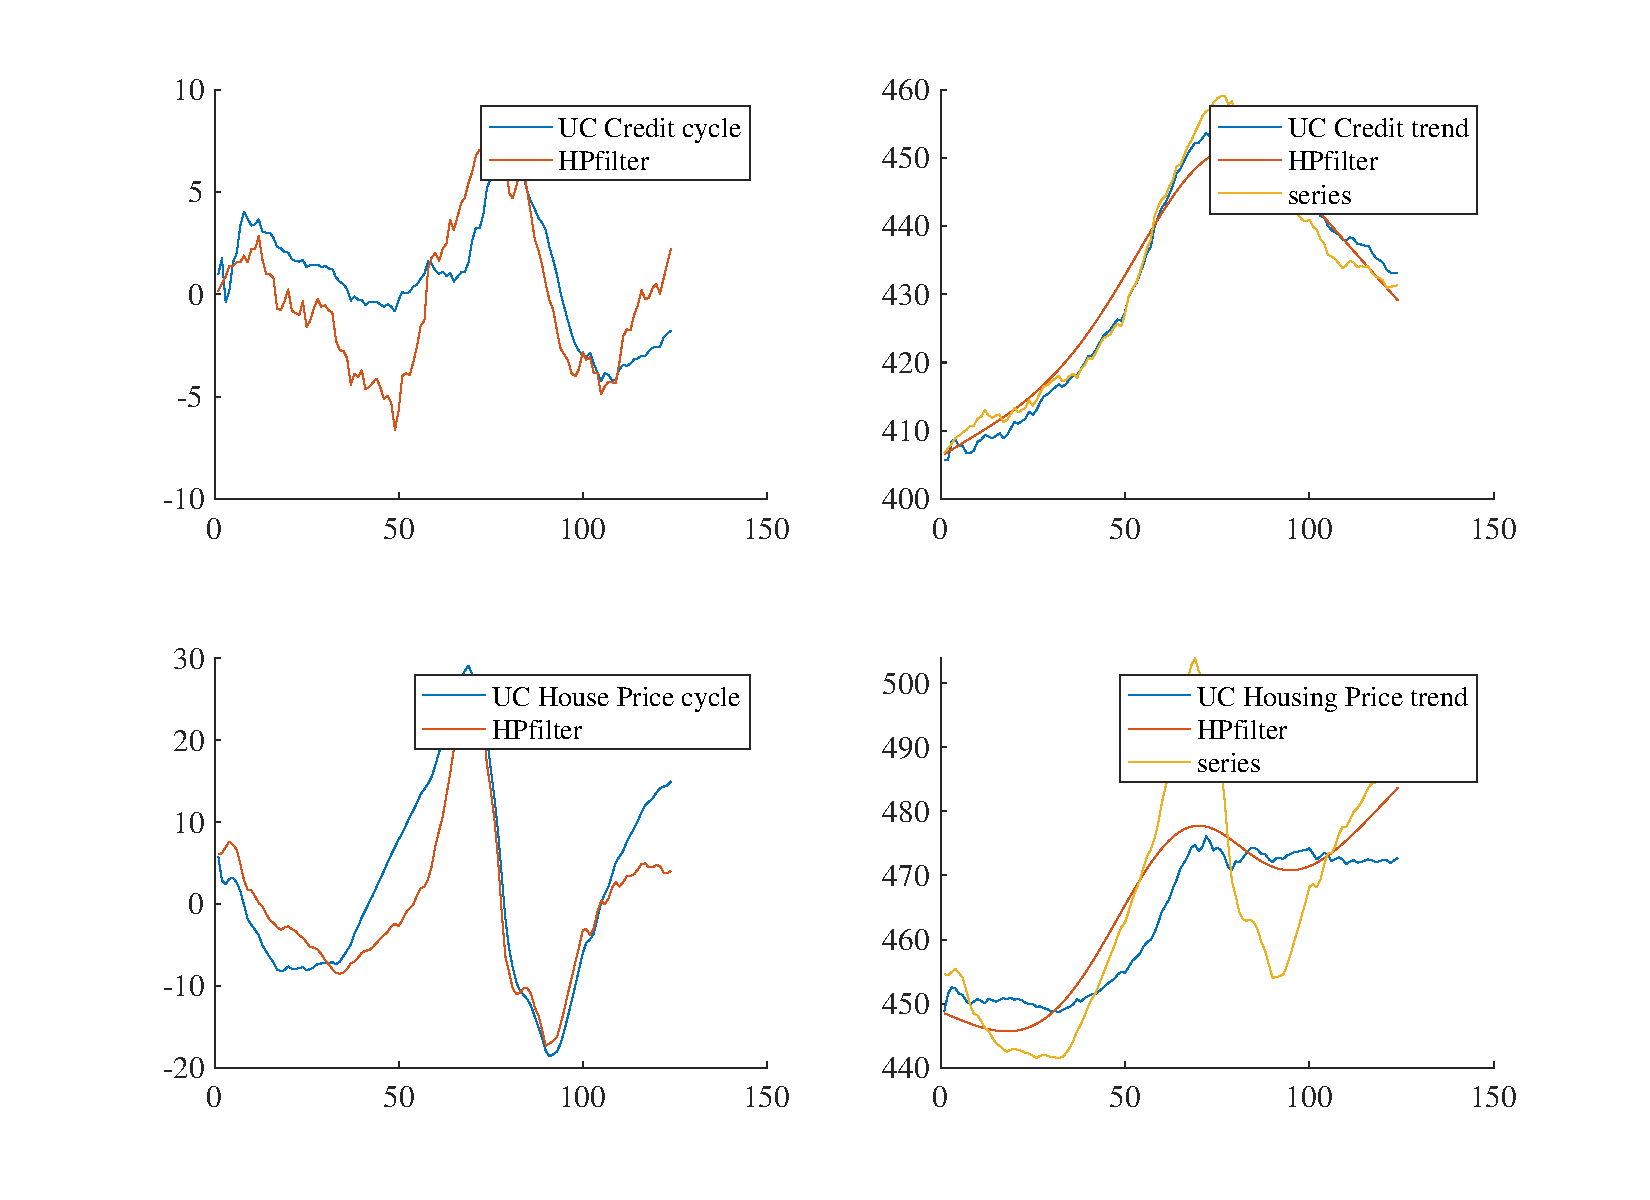
\includegraphics[width=0.85\linewidth]{../../Regression/Bayesian_UC_VAR2_drift_Crosscycle2lags/OutputData/cycles_US} 

}

\caption{US VAR(2) 2 cross-lags}\label{fig:unnamed-chunk-8}
\end{figure}

\clearpage

\hypertarget{posterior-and-prior-distribution}{%
\section{Posterior and Prior Distribution}\label{posterior-and-prior-distribution}}

\hypertarget{uk-posterior-and-prior-distribution}{%
\subsection{UK Posterior and Prior Distribution}\label{uk-posterior-and-prior-distribution}}

\begin{figure}

{\centering 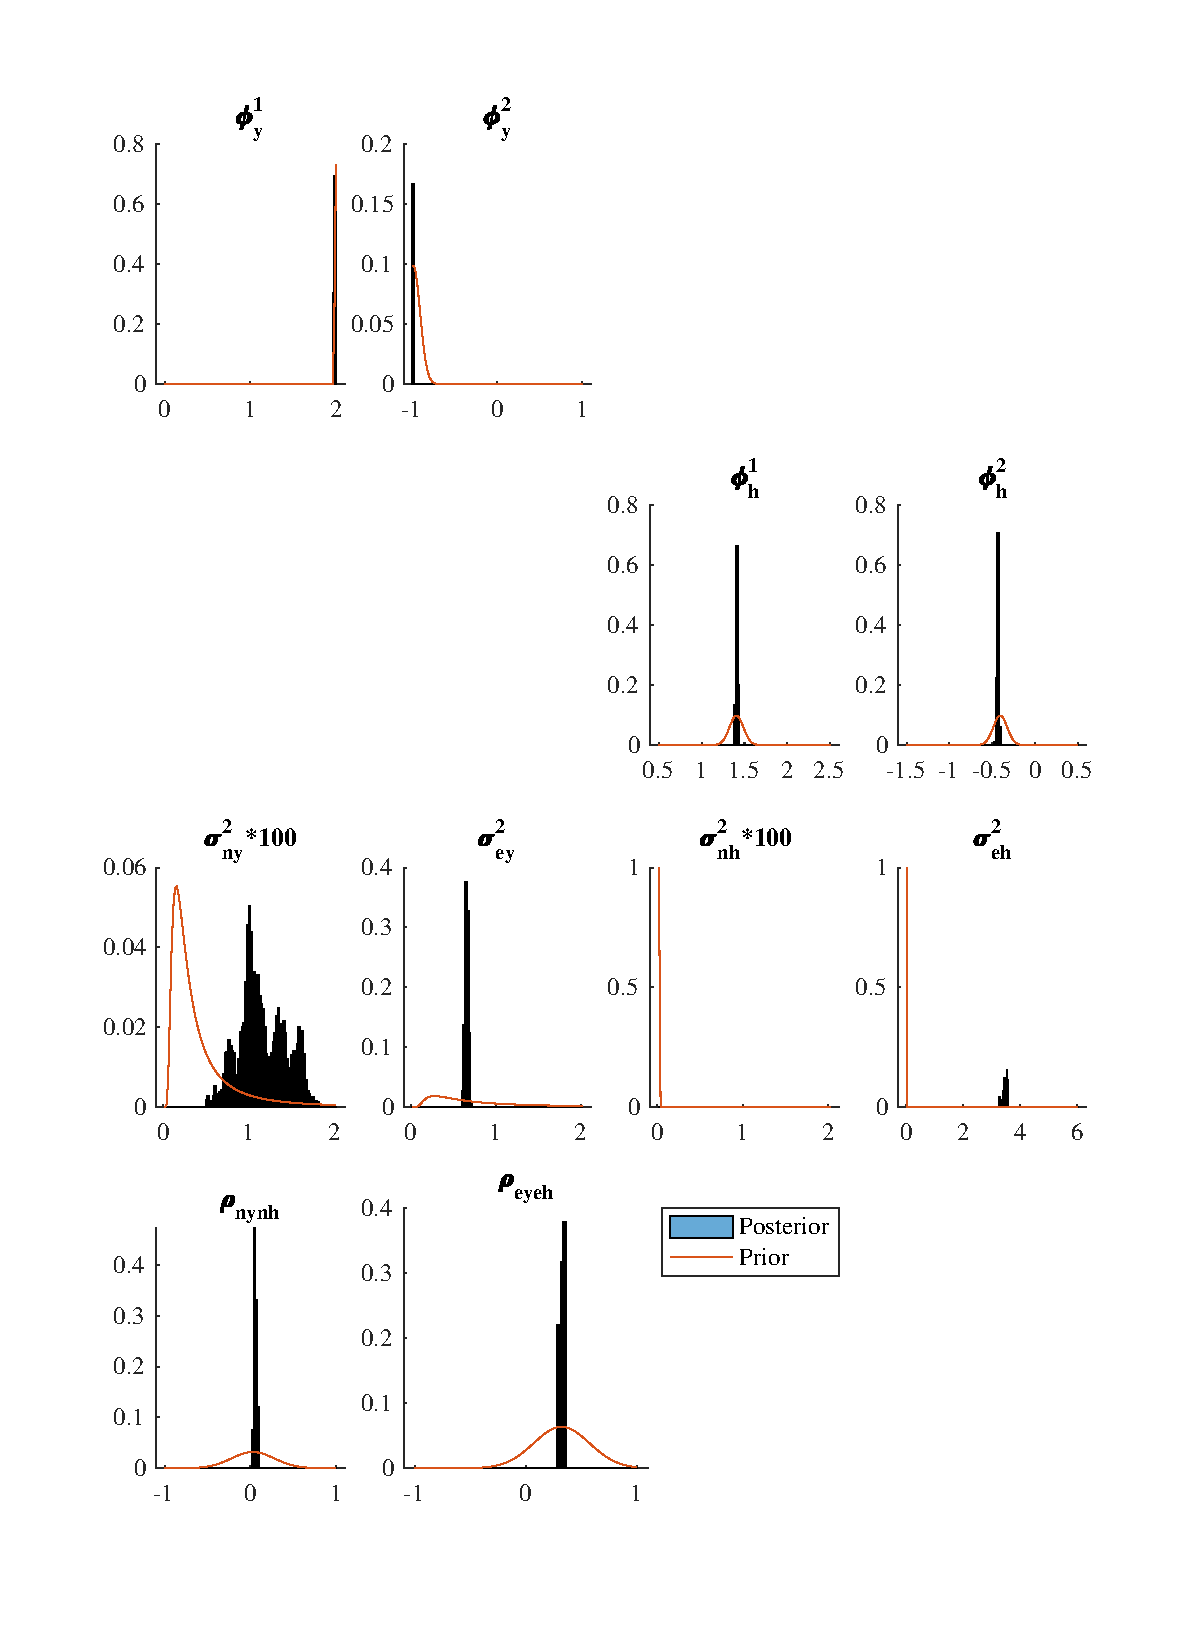
\includegraphics[width=0.85\linewidth]{../../Regression/Bayesian_UC_VAR2_drift/OutputData/posteriorpriordistribution_UK} 

}

\caption{UK VAR(2)}\label{fig:unnamed-chunk-9}
\end{figure}

\begin{figure}

{\centering 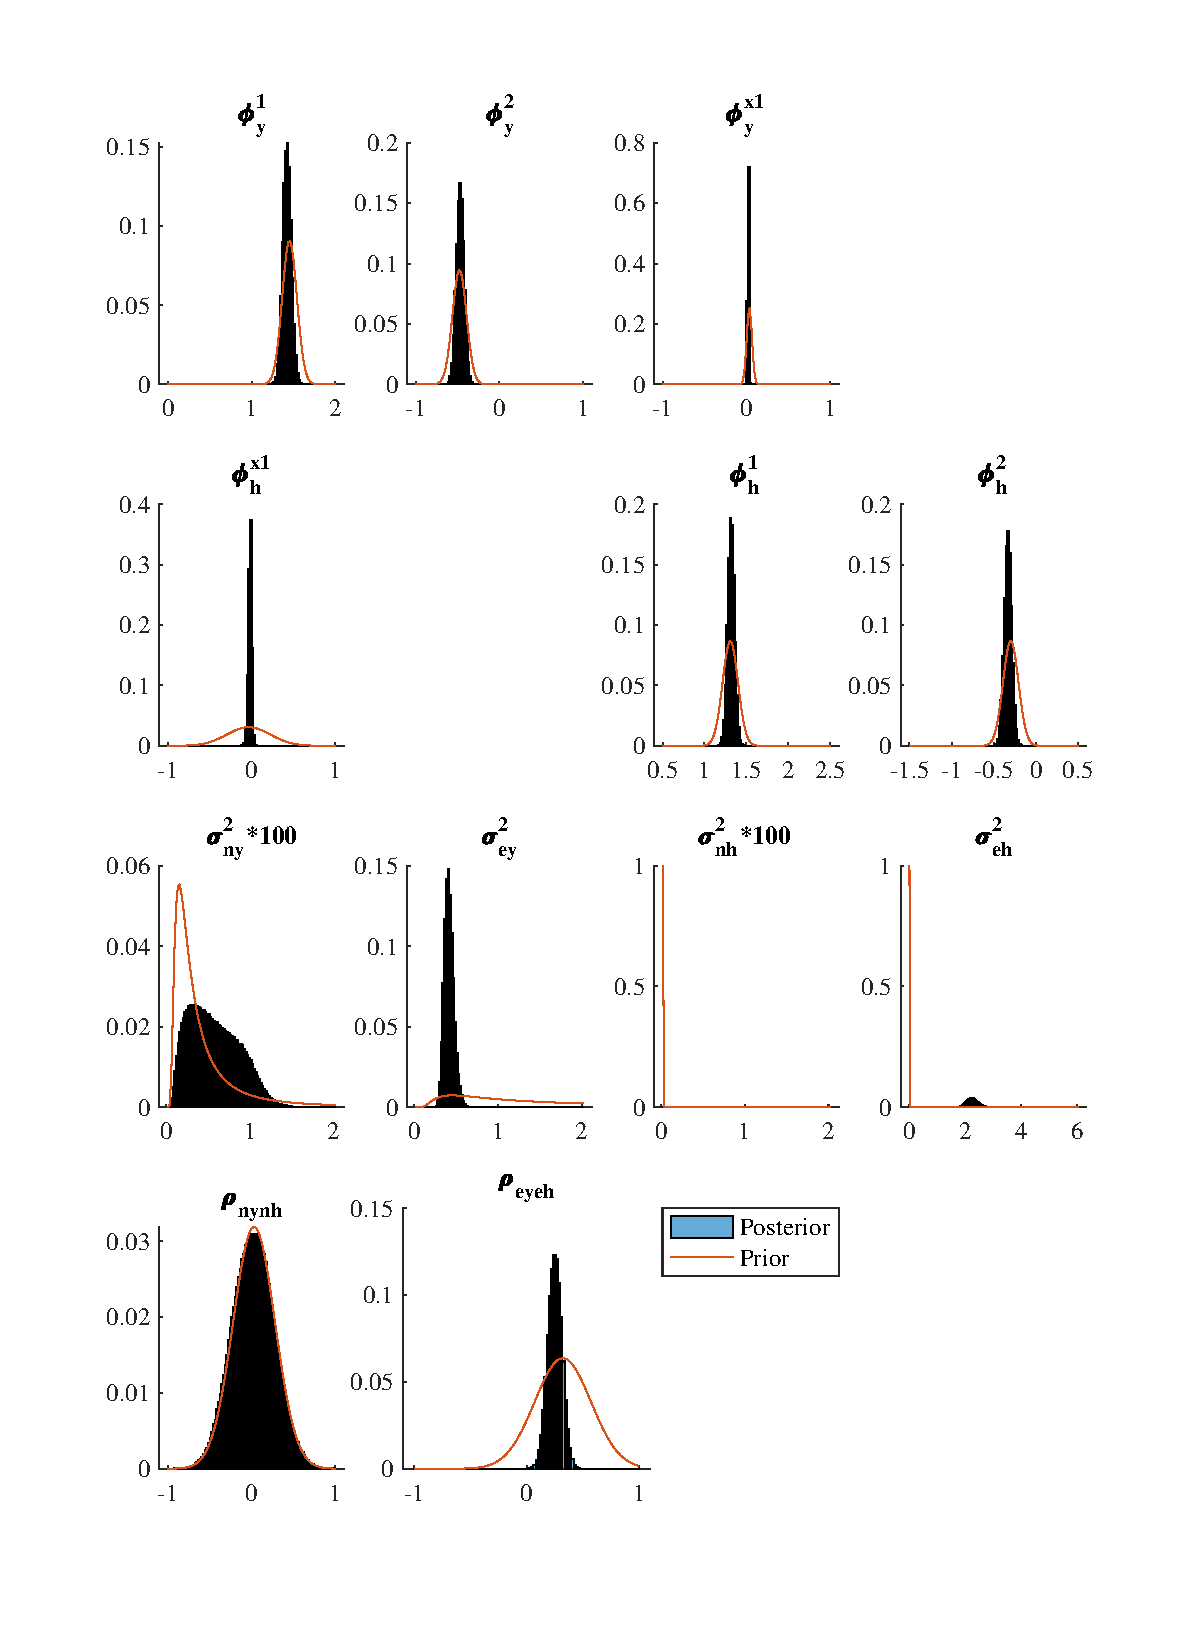
\includegraphics[width=0.85\linewidth]{../../Regression/Bayesian_UC_VAR2_drift_Crosscycle1lag/OutputData/posteriorpriordistribution_UK} 

}

\caption{UK VAR(2) 1 cross-lag}\label{fig:unnamed-chunk-10}
\end{figure}

\begin{figure}

{\centering 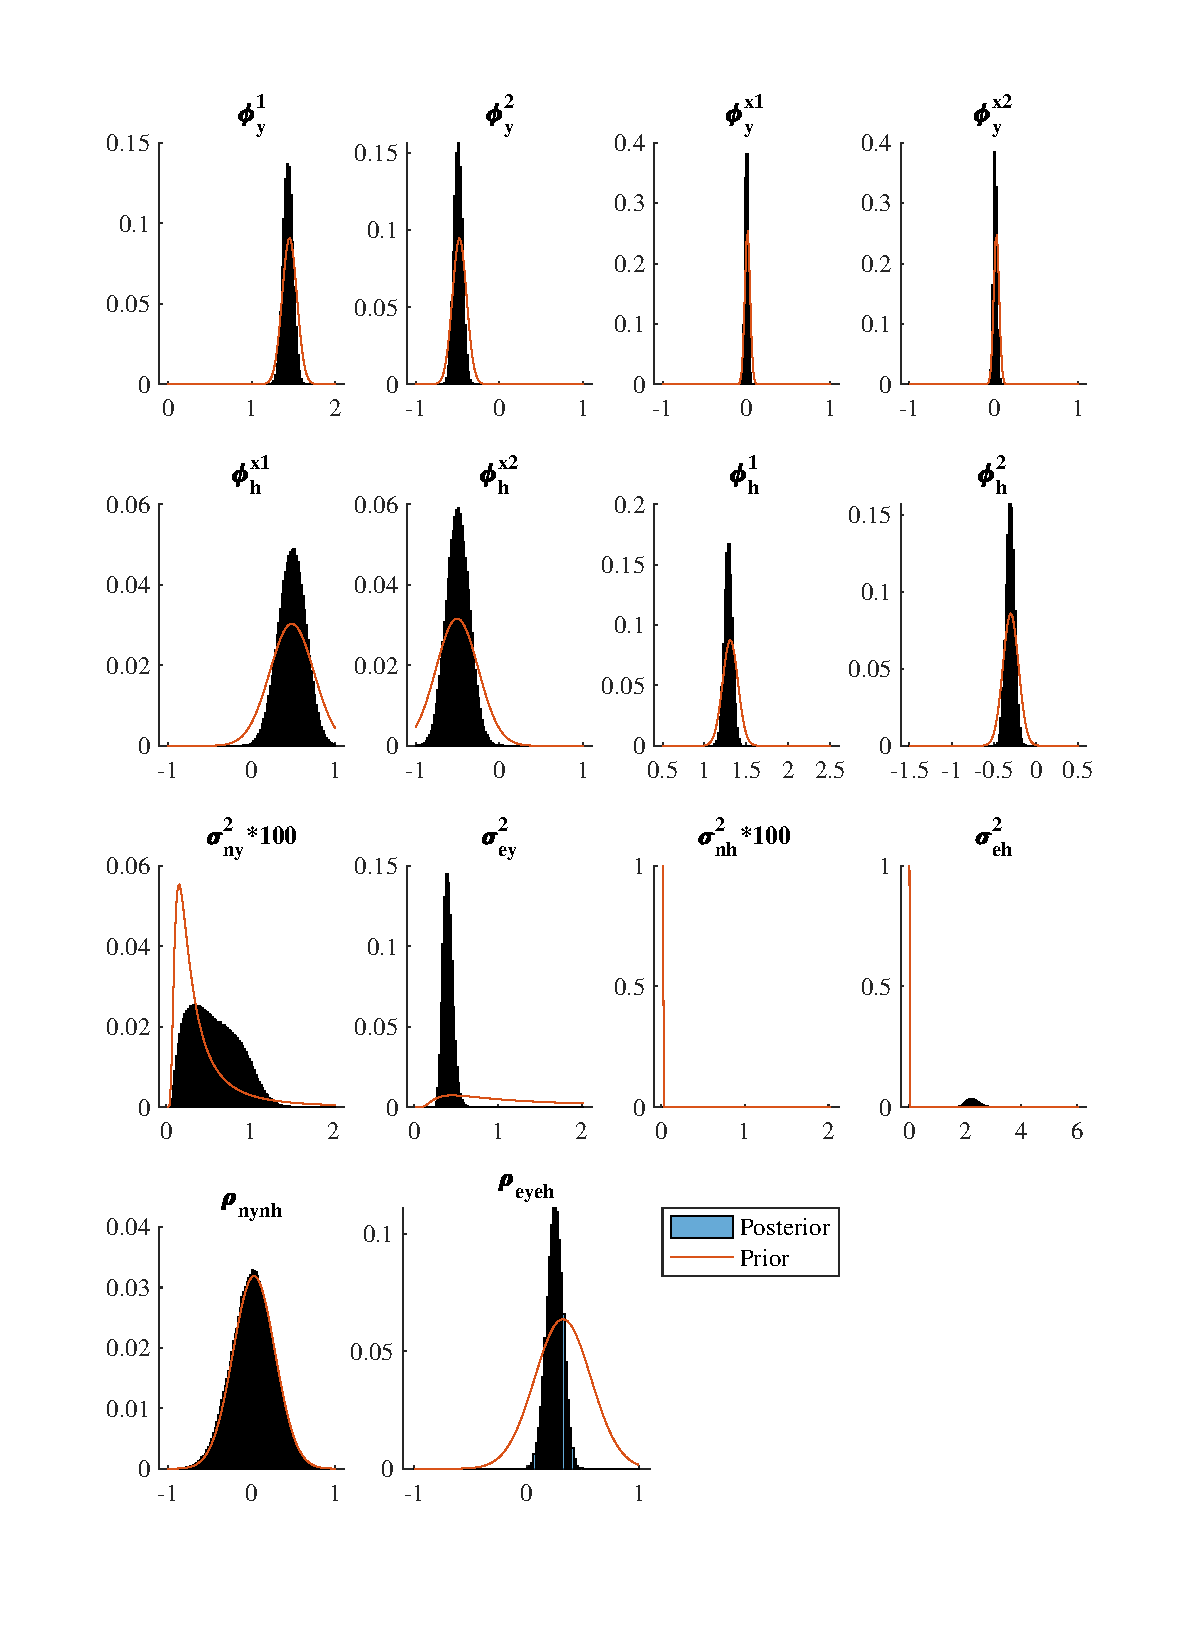
\includegraphics[width=0.85\linewidth]{../../Regression/Bayesian_UC_VAR2_drift_Crosscycle2lags/OutputData/posteriorpriordistribution_UK} 

}

\caption{UK VAR(2) 2 cross-lags}\label{fig:unnamed-chunk-11}
\end{figure}

\clearpage

\hypertarget{us-posterior-and-prior-distribution}{%
\subsection{US Posterior and Prior Distribution}\label{us-posterior-and-prior-distribution}}

\begin{figure}

{\centering 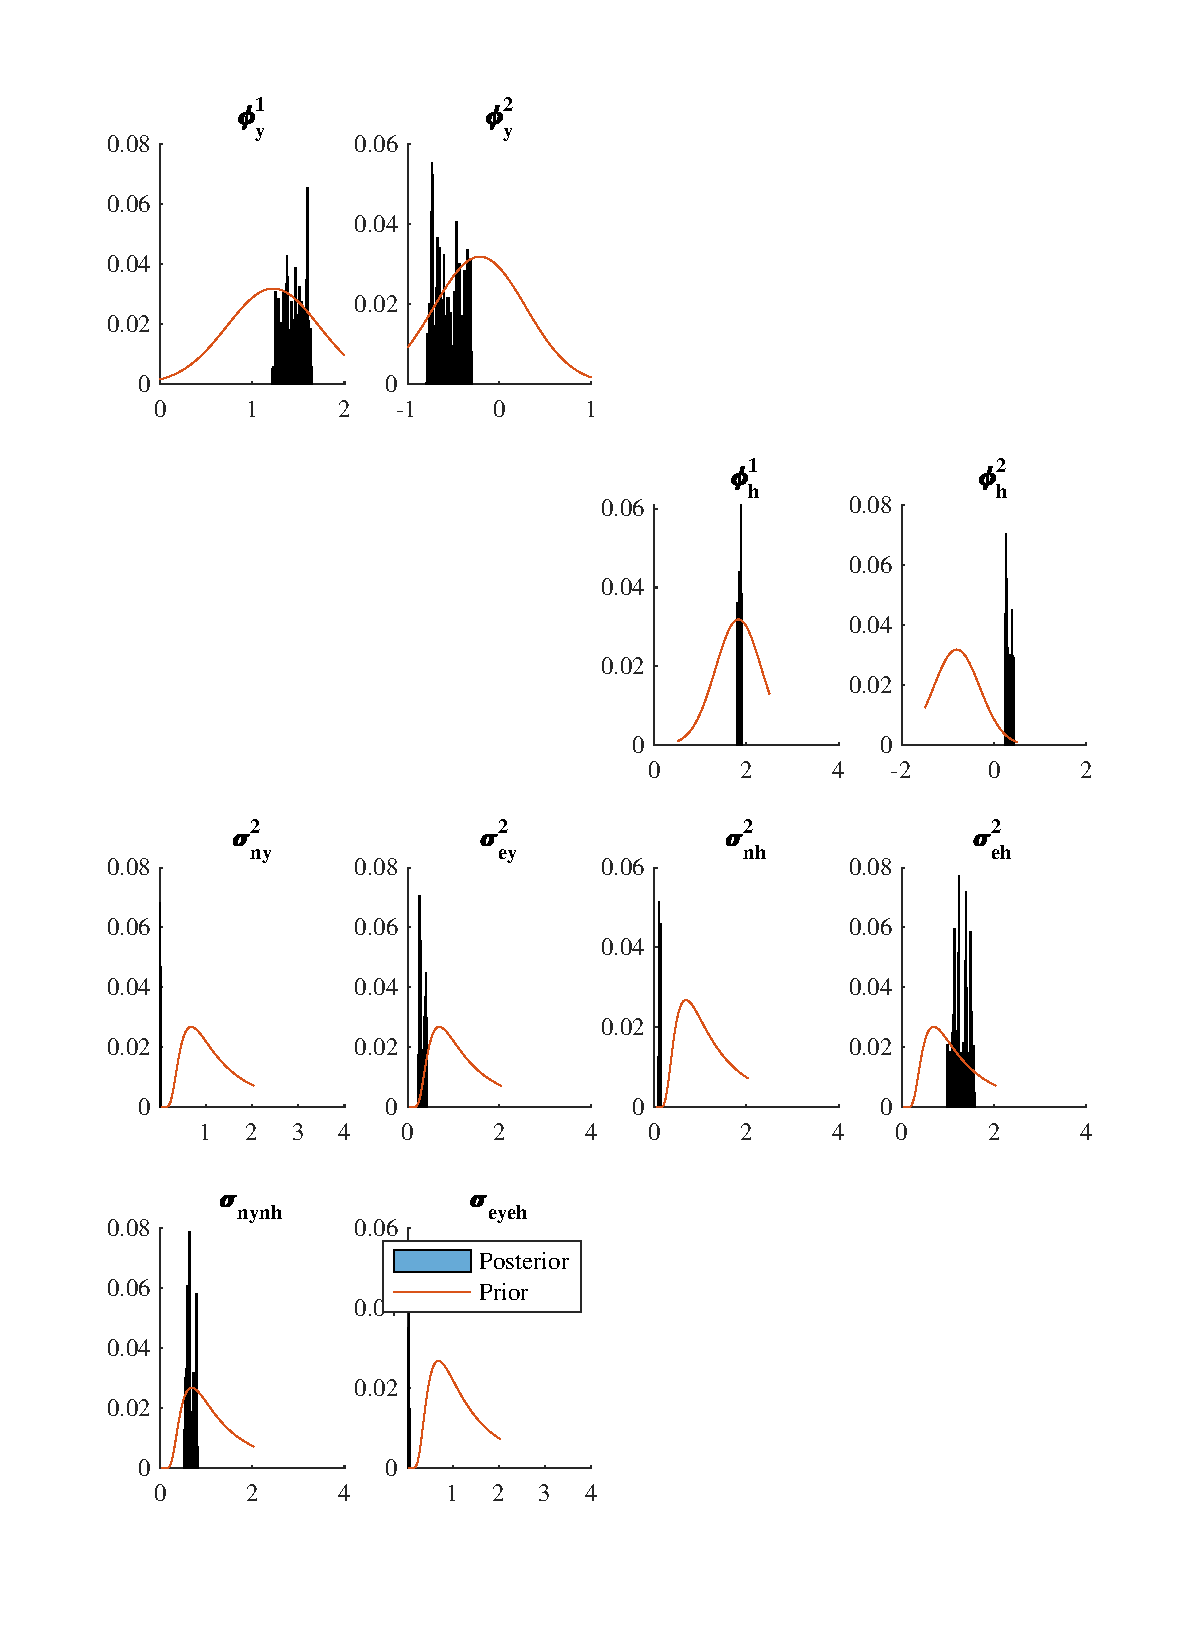
\includegraphics[width=0.85\linewidth]{../../Regression/Bayesian_UC_VAR2_drift/OutputData/posteriorpriordistribution_US} 

}

\caption{US VAR(2)}\label{fig:unnamed-chunk-12}
\end{figure}

\begin{figure}

{\centering 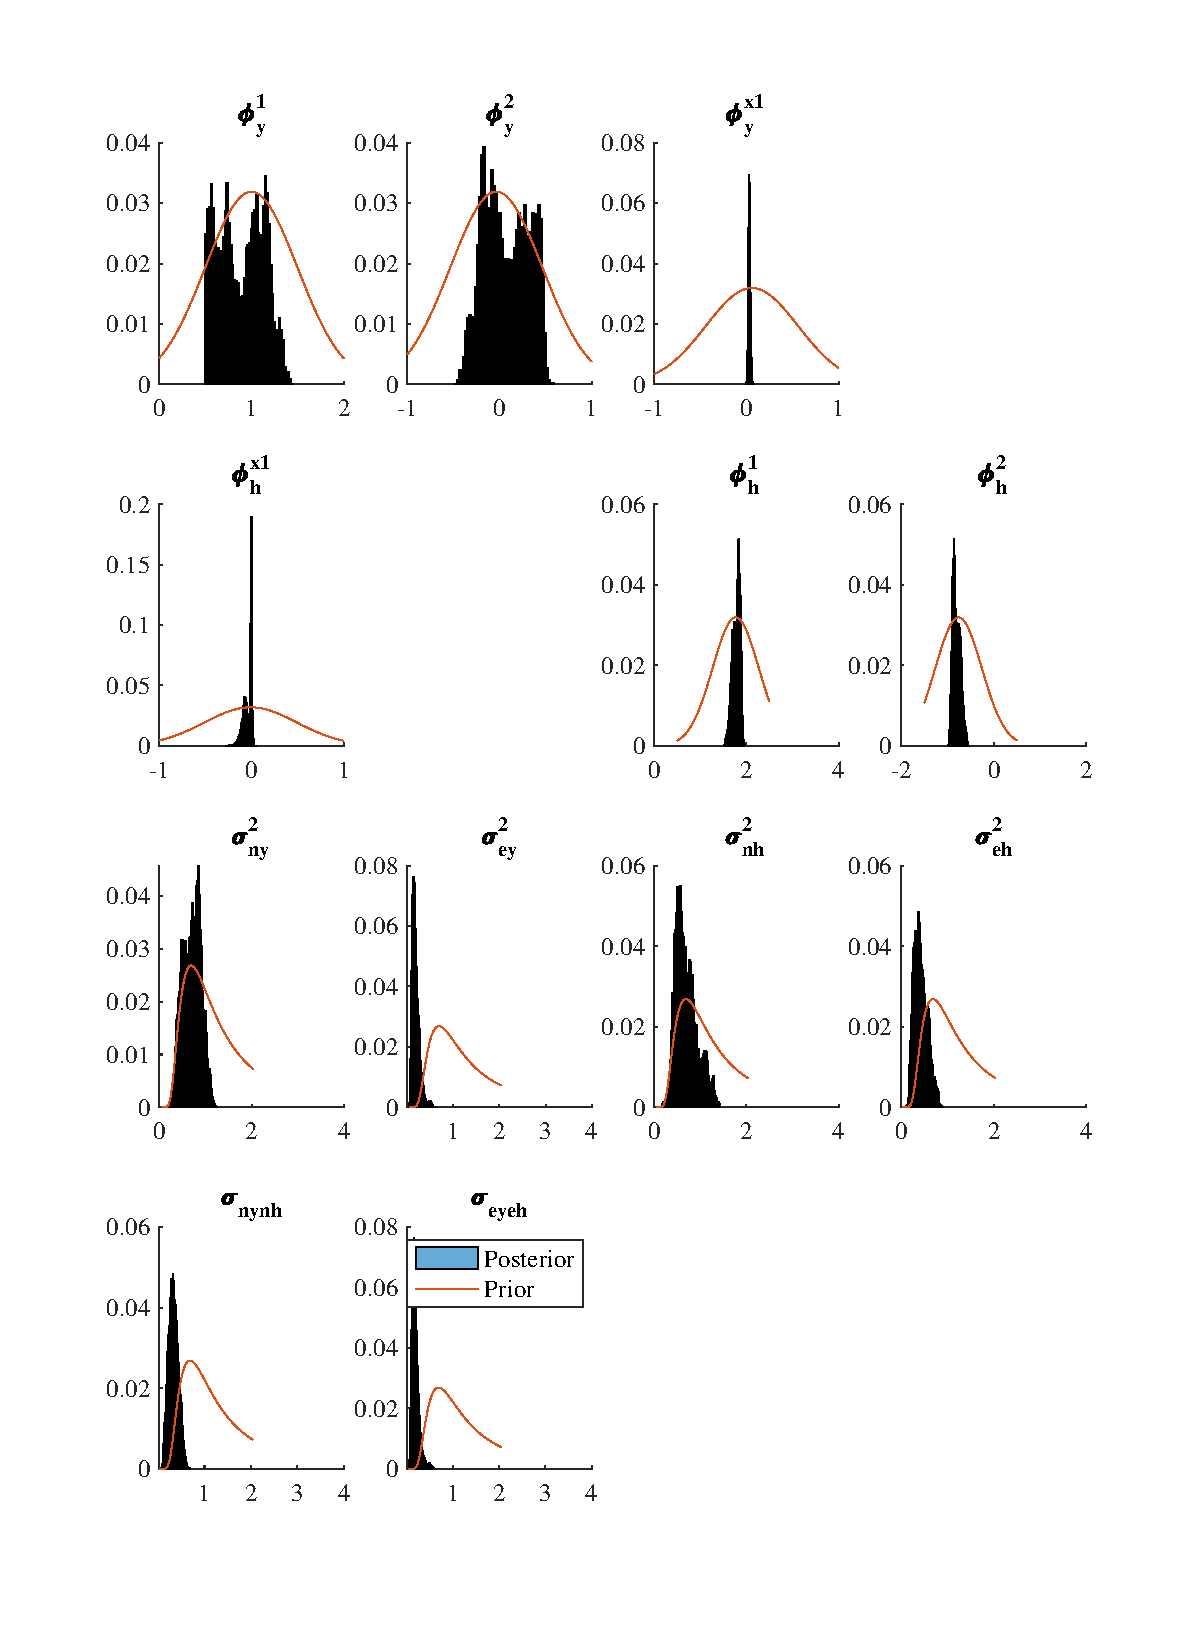
\includegraphics[width=0.85\linewidth]{../../Regression/Bayesian_UC_VAR2_drift_Crosscycle1lag/OutputData/posteriorpriordistribution_US} 

}

\caption{US VAR(2) 1 cross-lag}\label{fig:unnamed-chunk-13}
\end{figure}

\begin{figure}

{\centering 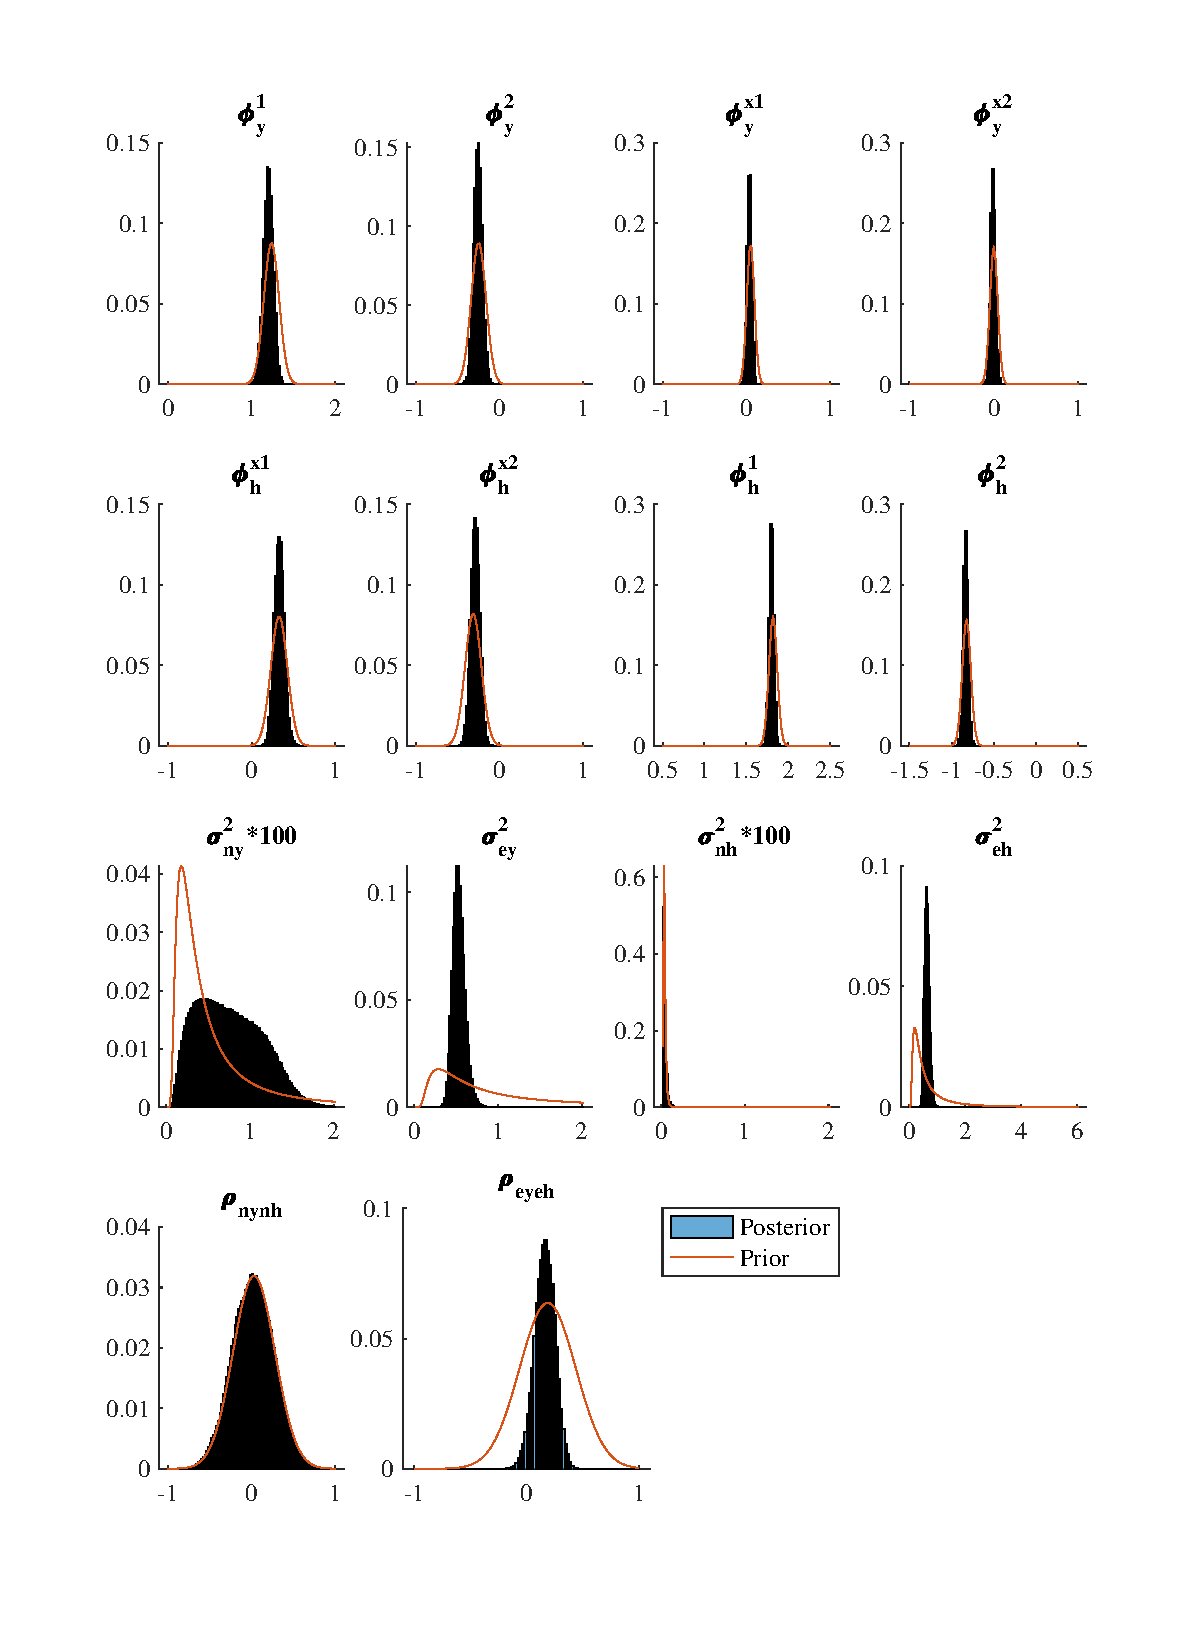
\includegraphics[width=0.85\linewidth]{../../Regression/Bayesian_UC_VAR2_drift_Crosscycle2lags/OutputData/posteriorpriordistribution_US} 

}

\caption{US VAR(2) 2 cross-lags}\label{fig:unnamed-chunk-14}
\end{figure}

\clearpage

\hypertarget{posterior-chain}{%
\section{Posterior chain}\label{posterior-chain}}

\hypertarget{uk-posterior-chain}{%
\subsection{UK Posterior chain}\label{uk-posterior-chain}}

\begin{figure}

{\centering 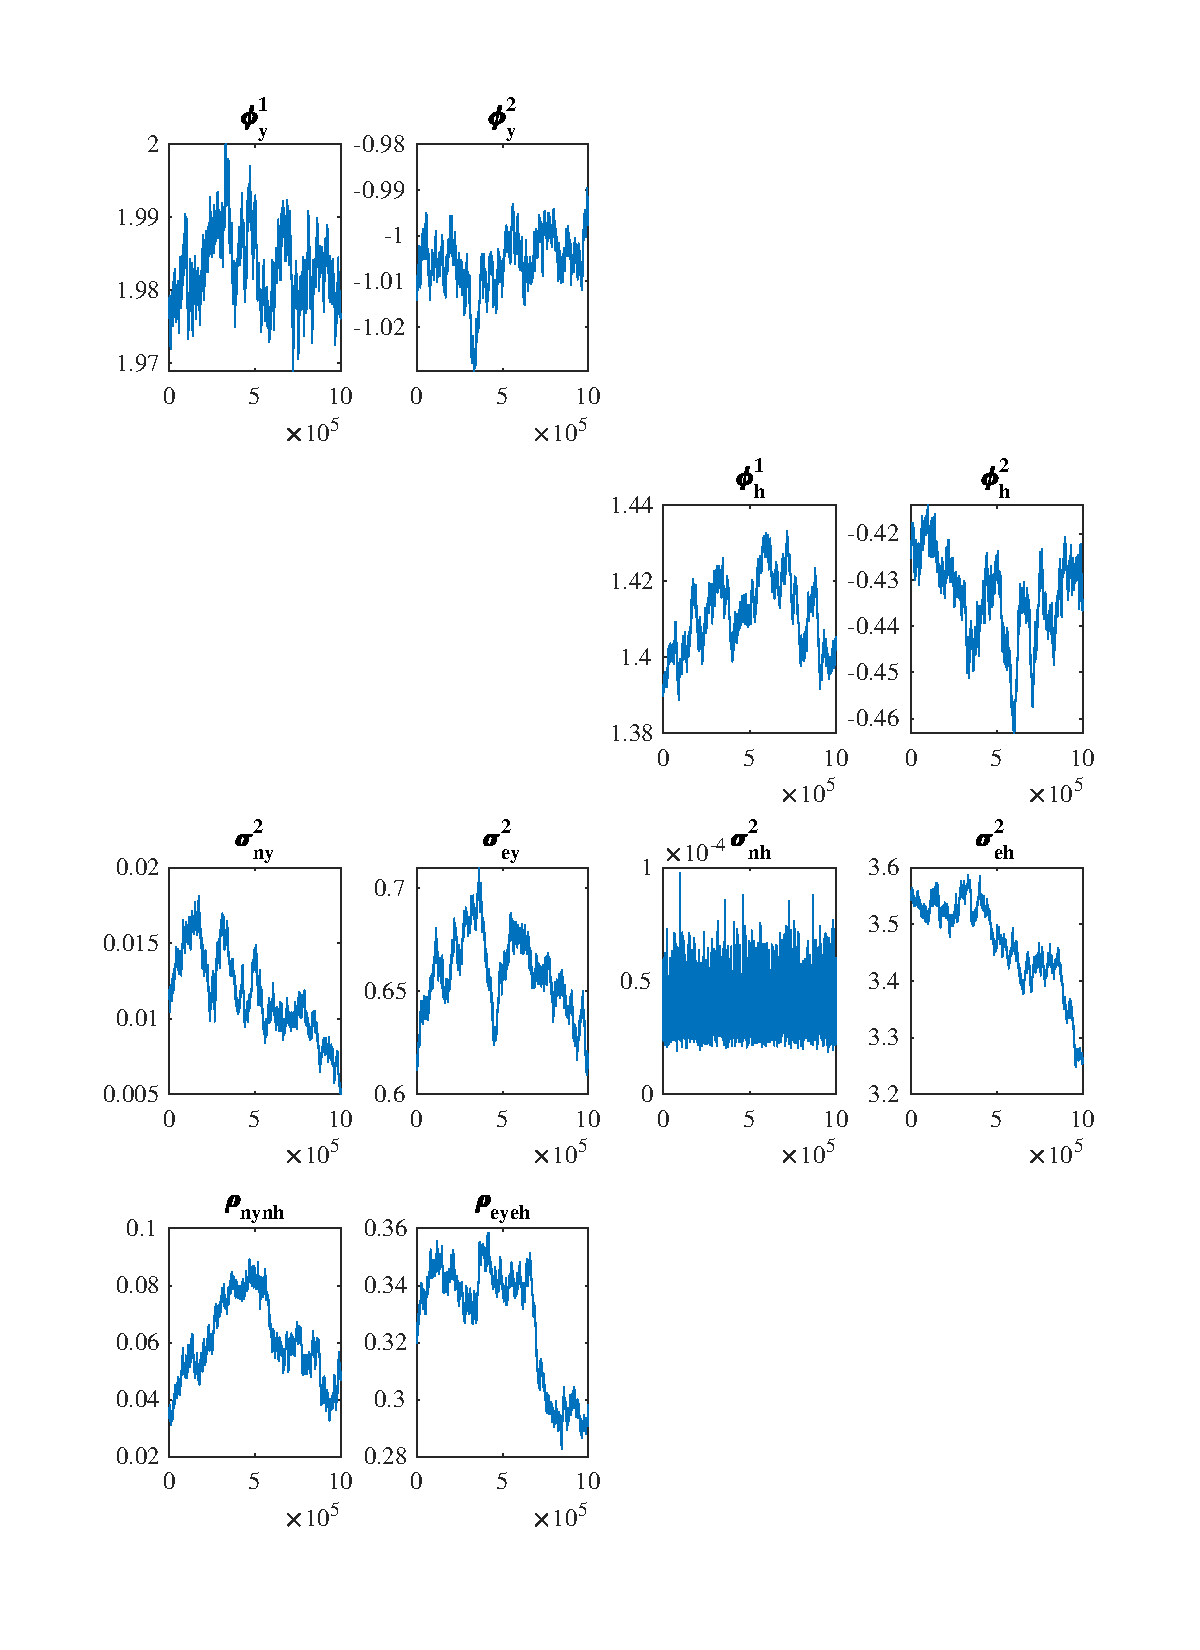
\includegraphics[width=0.85\linewidth]{../../Regression/Bayesian_UC_VAR2_drift/OutputData/posteriorchain_UK} 

}

\caption{UK VAR(2)}\label{fig:unnamed-chunk-15}
\end{figure}

\begin{figure}

{\centering 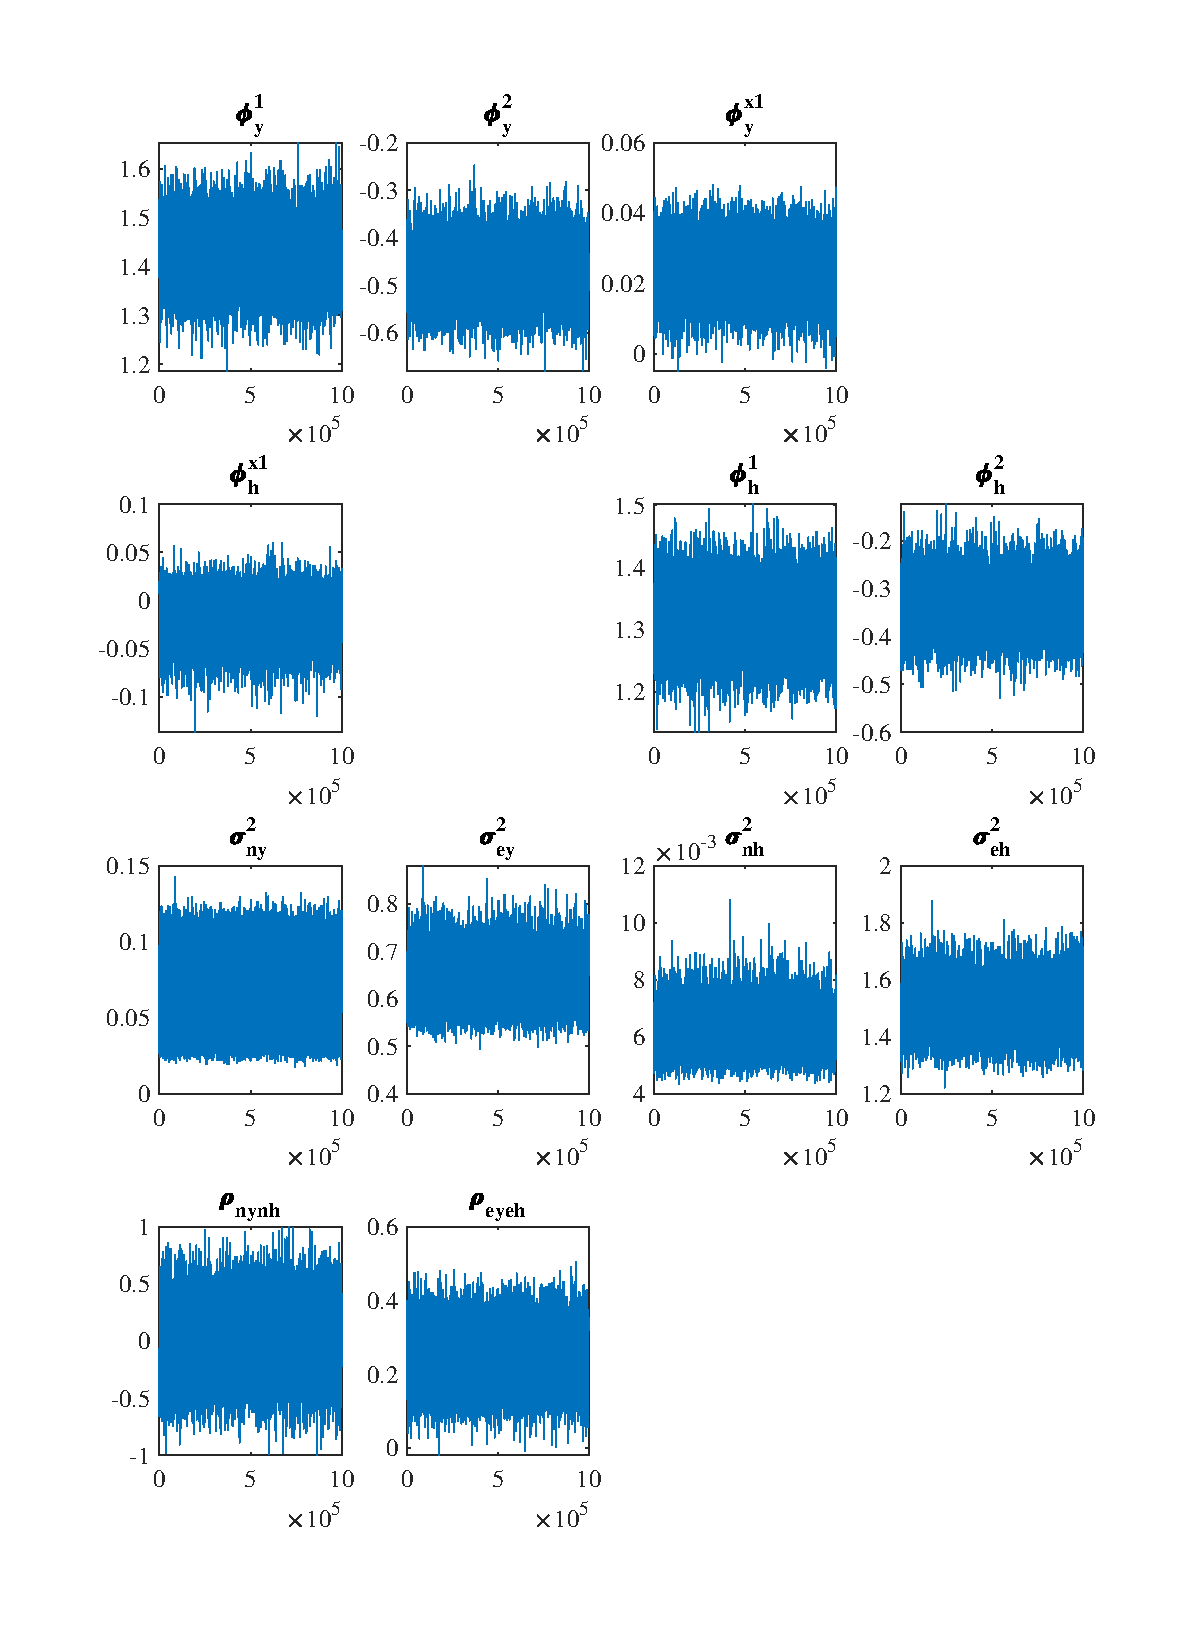
\includegraphics[width=0.85\linewidth]{../../Regression/Bayesian_UC_VAR2_drift_Crosscycle1lag/OutputData/posteriorchain_UK} 

}

\caption{UK VAR(2) 1 cross-lag}\label{fig:unnamed-chunk-16}
\end{figure}

\begin{figure}

{\centering 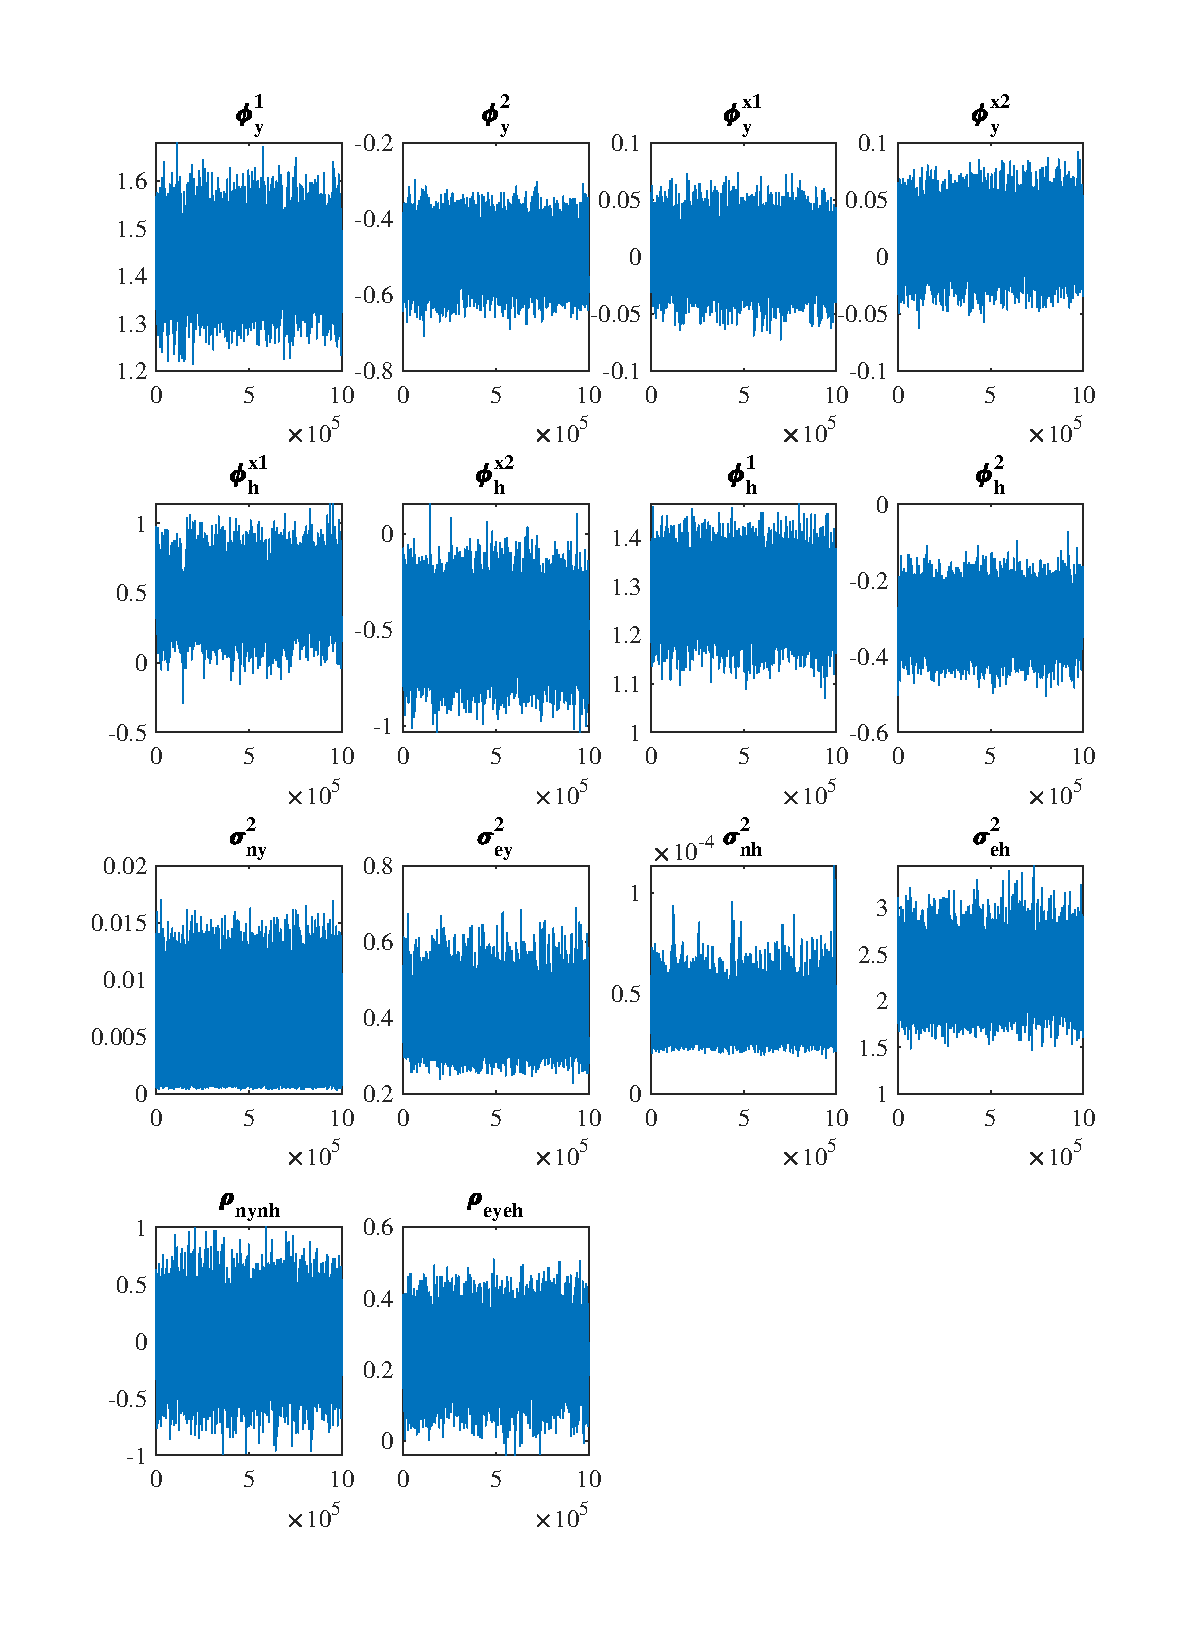
\includegraphics[width=0.85\linewidth]{../../Regression/Bayesian_UC_VAR2_drift_Crosscycle2lags/OutputData/posteriorchain_UK} 

}

\caption{UK VAR(2) 2 cross-lags}\label{fig:unnamed-chunk-17}
\end{figure}

\clearpage

\hypertarget{us-posterior-chain}{%
\subsection{US Posterior chain}\label{us-posterior-chain}}

\begin{figure}

{\centering 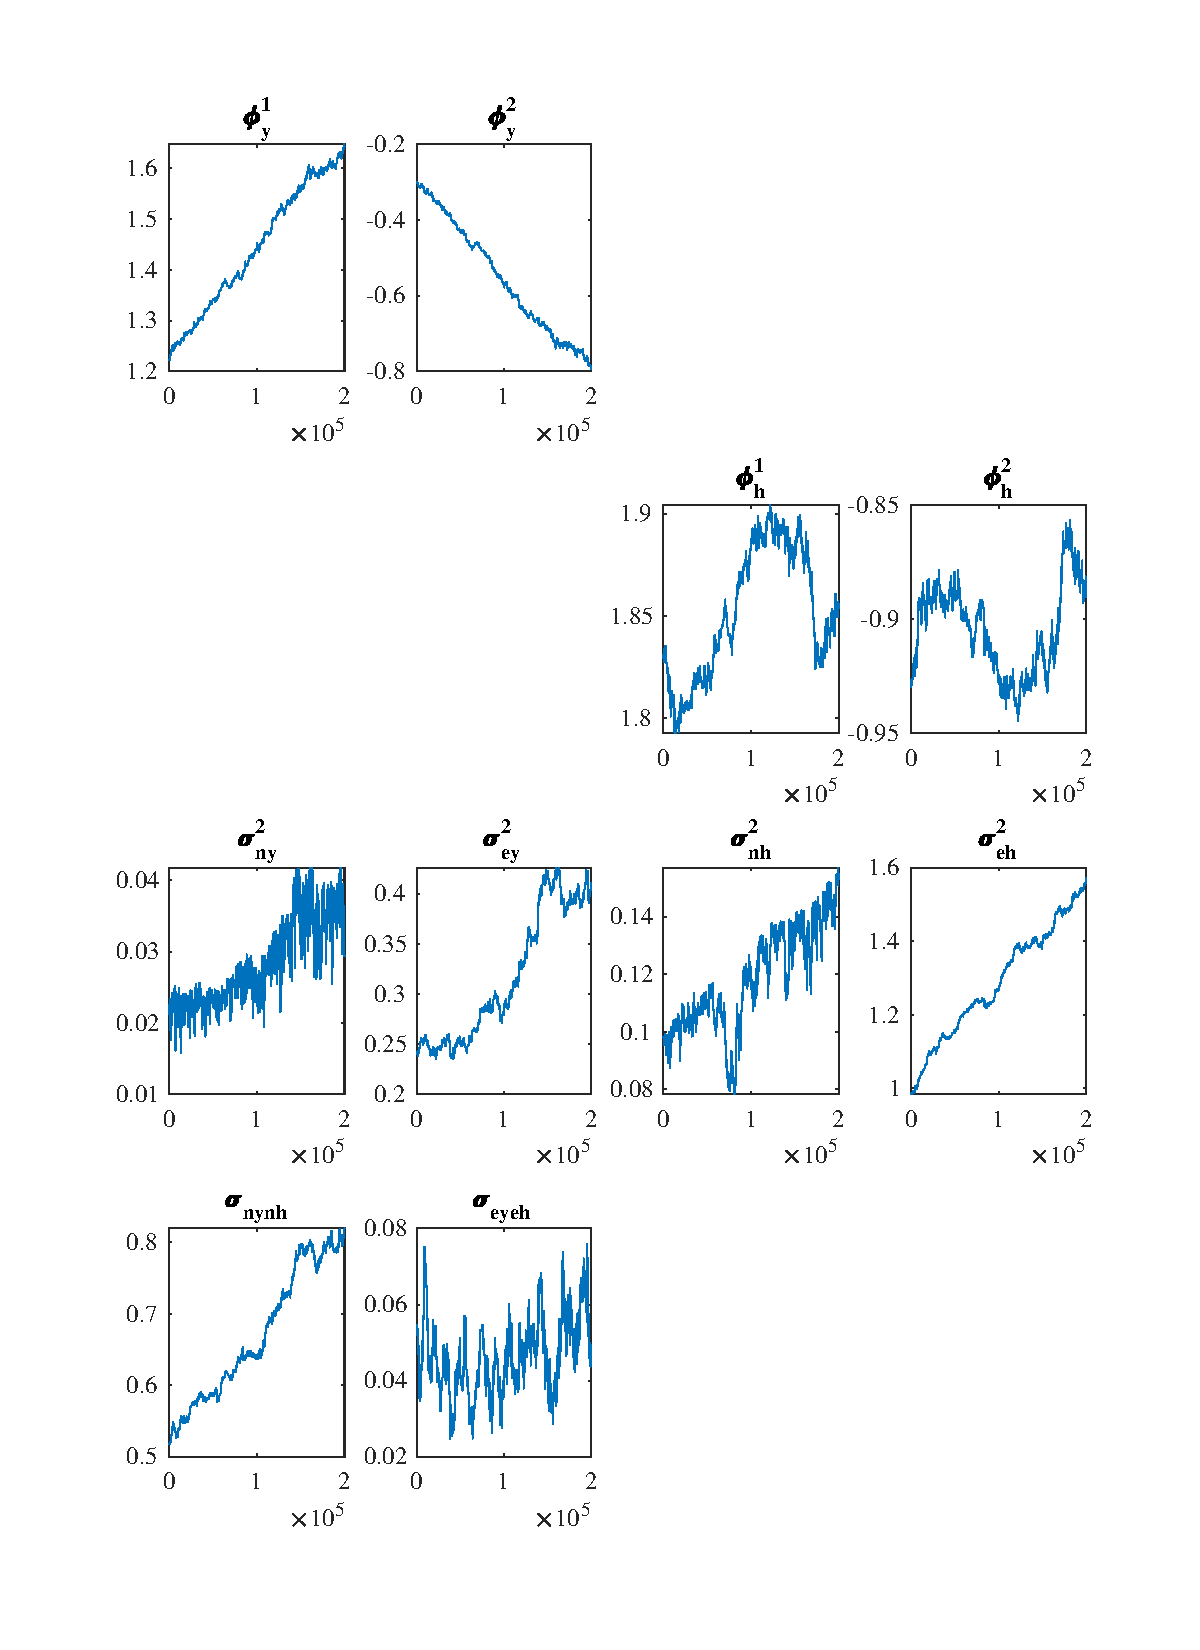
\includegraphics[width=0.85\linewidth]{../../Regression/Bayesian_UC_VAR2_drift/OutputData/posteriorchain_US} 

}

\caption{US VAR(2)}\label{fig:unnamed-chunk-18}
\end{figure}

\begin{figure}

{\centering 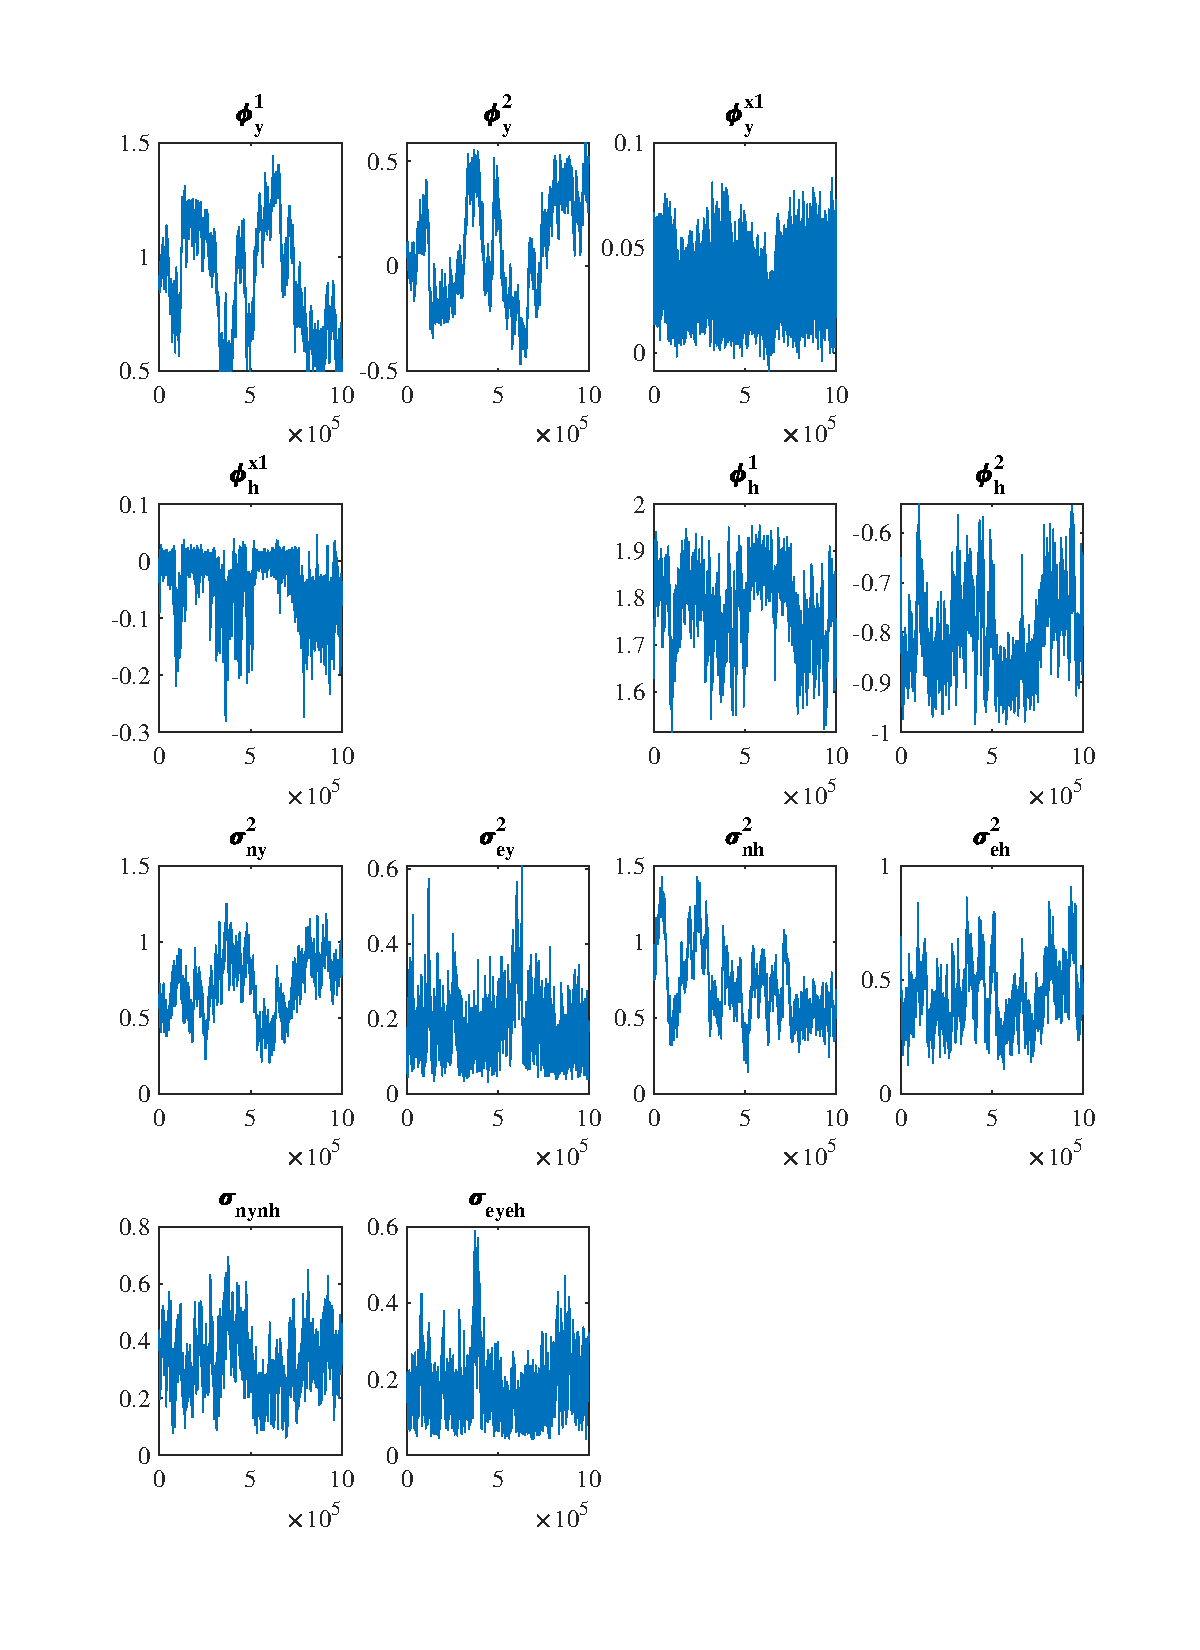
\includegraphics[width=0.85\linewidth]{../../Regression/Bayesian_UC_VAR2_drift_Crosscycle1lag/OutputData/posteriorchain_US} 

}

\caption{US VAR(2) 1 cross-lag}\label{fig:unnamed-chunk-19}
\end{figure}

\begin{figure}

{\centering 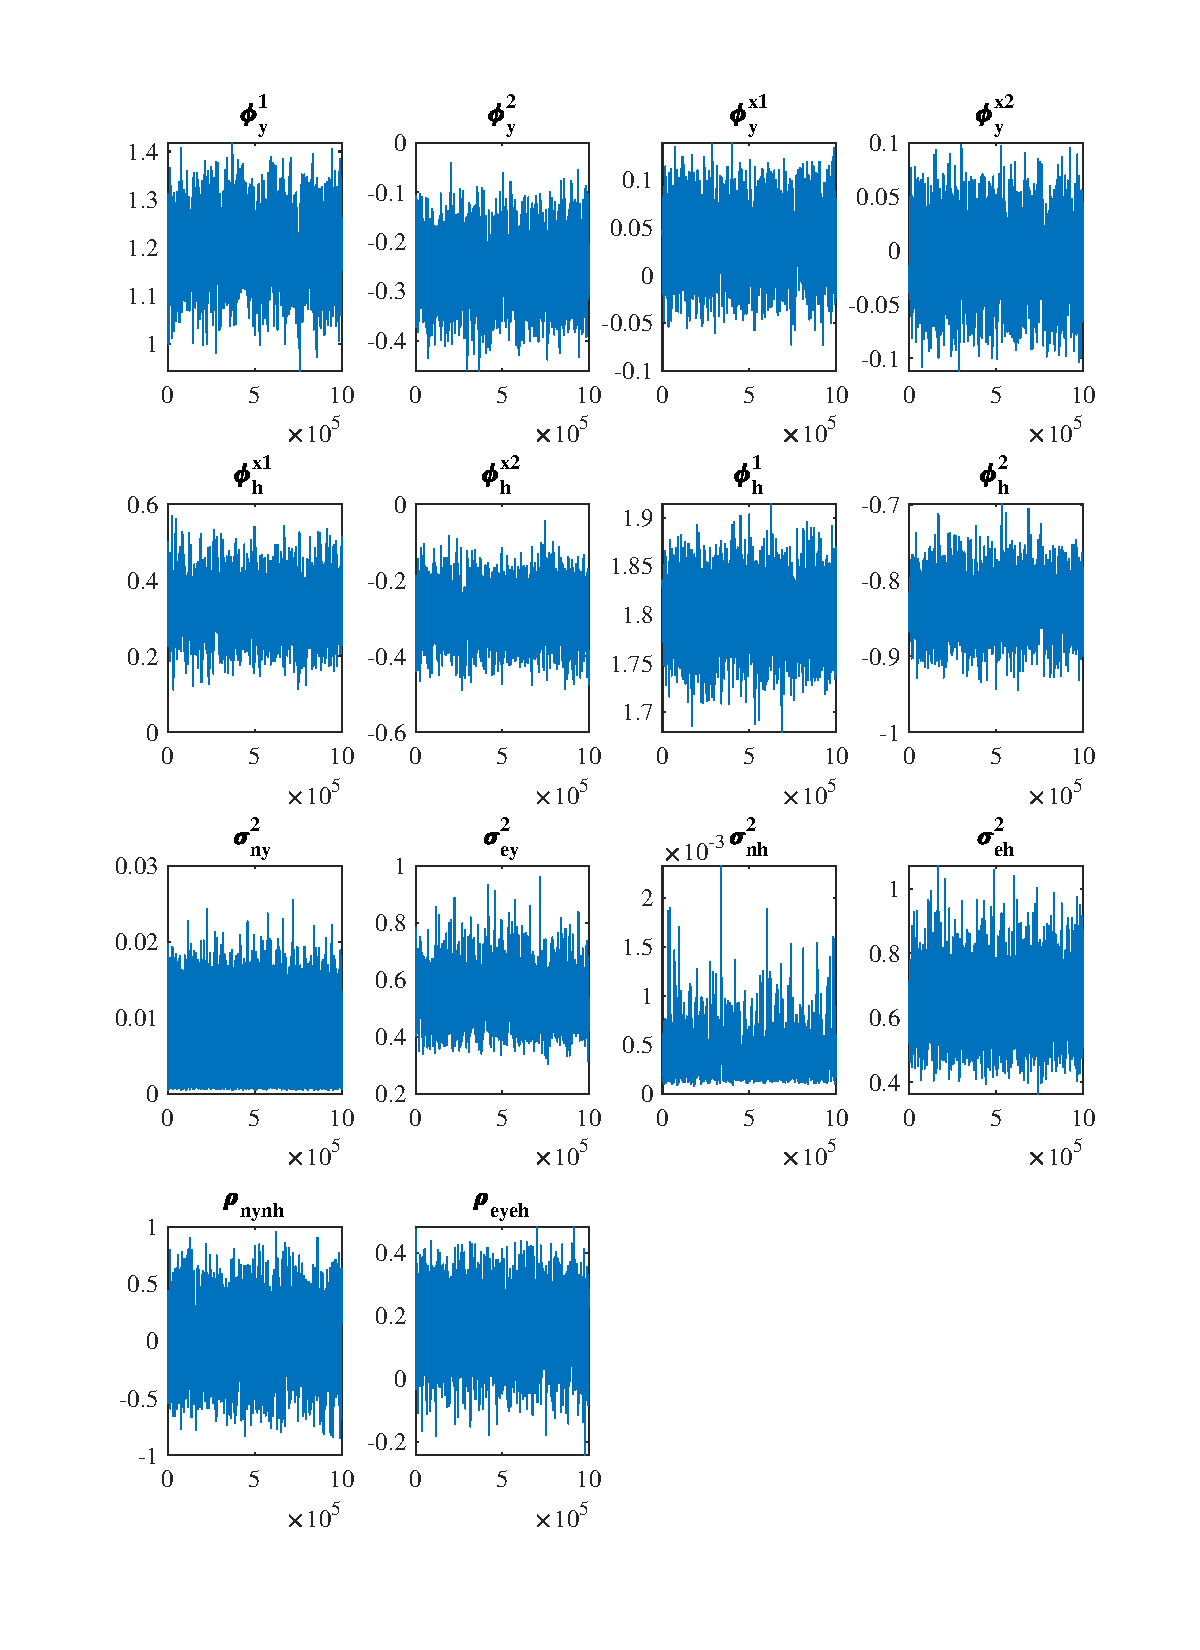
\includegraphics[width=0.85\linewidth]{../../Regression/Bayesian_UC_VAR2_drift_Crosscycle2lags/OutputData/posteriorchain_US} 

}

\caption{US VAR(2) 2 cross-lags}\label{fig:unnamed-chunk-20}
\end{figure}

\end{document}
